
%%\documentclass{article}
\documentclass{scrartcl}

%"First you tell 'em what you're going to tell 'em. Then you tell 'em. Then you tell 'em what you've told 'em."

\usepackage{multirow} % 24/10

%\usepackage[table]{xcolor}%10/20
%\arrayrulecolor{blue} %10/20
\usepackage{cmap}
\usepackage{booktabs}
\usepackage{colortbl}
\usepackage{multirow}
\usepackage{subfloat}
\usepackage{float}
\floatstyle{boxed} 
\restylefloat{figure}

\usepackage{caption}

\usepackage{lipsum}

\usepackage{kpfonts}

\usepackage{polyglossia}
\usepackage{csquotes}
\setdefaultlanguage{english}
%%%%%%%%%%%%%%%% for color
\usepackage{xcolor, colortbl} 
\newcommand{\mc}[2]{\multicolumn{#1}{c}{#2}}
\definecolor{Gray}{gray}{0.85}
\definecolor{LightCyan}{rgb}{0.88,1,1}

\newcolumntype{a}{>{\columncolor{Gray}}c}
\newcolumntype{b}{>{\columncolor{white}}c}
%%%%%%%%%%%%%%%%%%%%%%%%%%
%\usepackage[backend=biber]{biblatex}
\usepackage[backend=biber, style=ieee]{biblatex}
\addbibresource{plana.bib}

\usepackage{graphicx}
\graphicspath{ {images/} }

%%%% the package and hypersetup below make pdf clickable
\usepackage{hyperref}
\hypersetup{
    colorlinks,
    citecolor=black,
    filecolor=black,
    linkcolor=black,
    urlcolor=black
}
\hypersetup{linktocpage}






\begin{document}

\begin{titlepage}


\title{\textsc{\LARGE Bern University of Applied Sciences | BFH }\\[1cm]
\begin{center}
%
\includegraphics[width = 60mm]{logo.JPG}
\end{center}
\textsc{\small Department of Engineering and Information Technology}\\
\textsc{\small Bachelor's Thesis (BTI7321 ) Autumn Semester 2020/21}\\[1cm]
%\textsc{\small Report on  }\\
\textsc{"Planning of the Assignments for Lecturers(PLANA)" Web Application}}
\date{\today}   %% or \date{01 november 2019}
\author{\textit{Author: }Kristina \textsc{Shiryagina} (\texttt{kristina.shiryagina@bfh.ch}) \\
 \textit{Supervisor: } Prof. Marcel \textsc{Pfahrer}  (\texttt{marcel.pfahrer@bfh.ch})\\
 \textit{Expert: } Dr. Federico \textsc {Flueckiger}   \\
 }
\maketitle	

\newpage


	
\tableofcontents
\clearpage
\end{titlepage}

%%%%%%%%%% end title page
\setcounter{secnumdepth}{-2}% default for "report" is 2





\section{Acknowledgments}
%%I would like to thank my project supervisor - Prof. Marcel Pfahrer for his advice and guidance. 
%%I would also like to thank Andrei Herasimau for his corrections and Egger Samuel Sebastian for his advice.


\section{Abstract}


\setcounter{secnumdepth}{2}  % to make sections without numbers



\section{Introduction}
At our school at the Department of Technology and Computer Science, actual teacher assignment planning is done using Microsoft Excel tool.
This plan is handled by one responsible person.
The modern world with the rapid growth of new technologies makes it possible to improve various systems, giving them more and more possibilities, automating many functions and saving a lot of time.
This work aims to develop an information system that enables assignment planning for lecturers. But unlike the existing system, it should have the following criteria:
\begin{itemize}
\item the teachers themselves should be involved in the planning process
\item increased planning flexibility
\end{itemize}




Users of this system are the \textbf{study director} and \textbf{teachers}. Such planning implies collaborative work.
The planning process involves the input of specific data for specific user-defined views for each user and time limits set by the system. 

 All of these requirements need a more suitable system than Excel.
In the previous project, we compared \textbf{Microsoft Excel} and \textbf{Web Application} according to several criteria. And we concluded that the web application meets the requirements of the conceived system. The web application is designed to involve \textbf{many users}, it can have a  database that gives us \textbf{consistency of the data}. Also, the data is much \textbf{safer} in a database. The web application gives the best \textbf{overview} of the entire system. Comparing \textbf{desktop application} with \textbf{web application} web application wins in:
\begin{itemize}
\item it is accessible anywhere
\item no update needed 
\item costs less 
\end{itemize} 
 We decided to make a web application that will meet all the requirements and will be created using suitable modern technologies. Technologies such as ASP.NET Core Blazor Server with Entity Framework Core (EFCore) and MS SQL (Microsoft Structured Query Language) for the database were chosen. ASP.NET Core Blazor is a new framework that is gaining popularity. Interestingly, thanks to it, it becomes possible to do the entire application in C\# without using JavaScript.\\
This work is a continuation of a project that was completed last semester, In which we have prepared the necessary environment for this project.
In project 2, we created a prototype. In this work, the system will be detailed and expanded. In particular, the following goals are pursued:
\begin{itemize}
\item \textbf{Involvement of lecturers in the planning process.}
Lecturers can create their medium- and long-term plans in form of requests and proposal for the definite plan, which is then approved by the person responsible for the planning.
\item \textbf{Manage planning data.} Each teacher can manage his assignments.
\item \textbf{Grouping of lecturers.} It should be possible to schedule several lecturers for the same module.
   \begin{itemize}
   \item Teachers who join a group can independently manage their assignments related to their common module.
   \item Each teacher can make a group with other lecturers.
   \end{itemize}
 \item \textbf{Grouping of the modules.} The group of lecturers can choose the group of modules and set themselves to it. This can be done in the form of a proposal for the definitive plan, which is then approved by the person responsible for the planning.
\end{itemize}


 
In this work, first, we will explain how the project was organized and how we used a SCRUM to manage it, then we carry out an additional analysis of the system in connection with the expansion of the system requirements. We will make changes to the domain analysis. We will expand the topic of System Architecture and System Design. And then we will cover the topics Project Implementation and Testing.





%\section{Customer Problem Statement}
%
%\subsection{Problem Statement}


%\**
%A minimum 3-page high-level narrative about your project. The narrative should not be written from the developer’s perspective, describing the features of the planned system.
%Rather, put yourself into a customer’s role, and write your problem statement as if your imagined customer would write it! —Describe the problem that your customer is facing and his or her suggestions about how a software system could help.
%Your problem statement should be based on your project proposal, revised and improved as necessary.
%*\

\pagebreak

\subsection{Acronyms}	
\begin{table}[h]

%\begin{center}
\begin{tabular}{ p{2.5cm}| p{9.5cm} }
\rowcolor{LightCyan}
\hline
\textbf{Acronyms} & \textbf{Words} \\
\hline
EF                   &   Entity Framework\\ 
CSS      & Cascading Style Sheet \\ 
KKK      &              345\\ 
\end{tabular}
%\end{center}
\caption{Caption2}
\label{table2}
\end{table}



\subsection{Glossary}
\begin{itemize}


\item \textbf{FURPS+}\cite{eeles2005capturing} is a system for classifying requirements.
\begin{itemize}
\item Functionality
\item Usability
\item Reliability
\item Performance
\item Supportability 
\end{itemize}


\item \textbf{ SignalIR} is a free and open-source software library for Microsoft ASP.NET that allows server code to send asynchronous notifications to client-side web applications. 

\item \textbf{Blazor} is a free and open-source web framework that enables developers to create web apps using C\# and HTML. It is being developed by Microsoft.

\item \textbf{EF Core} 

\item \textbf{HTML} HyperText Markup language


\item \textbf{SQL} Structured Query Language
\item \textbf{JS } JavaScript
\item \textbf{CRUD} Create, read, update and delete
\item \textbf{UI} User Interface
\item \textbf{API} Application Programming Interface 

\item \textbf{MS} Microsoft
\item \textbf{BPMN} Business Process Model and Notation



\end{itemize}
%\section{System Requirements}

\section{Project Management}
\subsection{Effort Estimation}
  		
The Bachelor's Thesis  is designed as a 12 ECTS module. This corresponds to a workload of 360 hours. When we are working on a project, we always record our hours of work in an Excel table.
 At the end of the project, we will compare this time with the time allotted for the project. 		
  		
  		
  		
  		
  		
\subsection{Scrum}  	
The foundation of the project organization was Scrum.
 	    Some principles of Scrum could not be achieved since they need a group of more than two people. 
 	    Our work was based on the principles of Scrum like the Empirical Process of Control, the core of Scrum, self-organization, value-based prioritization, etc.
 	    The Empirical Process of Control includes three main ideas, namely transparency, inspection, and adaptation. \\
 	    Transparency: The work is carried out in full trust of all parties involved. Everyone has the courage to keep each other up to date with both good and bad news. \\ 
 	    Inspection: Inspection is carried out by every one in the Scrum Team. The team openly shows the product at the end of each Sprint.			 \\
 	    Adaptation: The team asks constant questions about the progress of work, whether we are on the right way. Depending on this, we can adapt an existing product.		 \\
 	    
 	    At the beginning of the project, we have discussed and estimated all the work that needs to be done. 
 	    Meetings between supervisor and developer are bi-weekly and sometimes weekly.
 	    Each meeting includes a discussion about what has been achieved 
 	    since the tasks have been assigned, what can be improved, and scheduling of future tasks.
 	    
 	    
 	    
 	    
 	    
 \subsubsection{Scrum Roles}
 \begin{itemize}
 \item Product Owner: Mr. Pfahrer
 \item Development Team: Shiryagina Kristina
 \item Scrum Master: Shiryagina Kristina
  		
  		\end{itemize}
  	    \subsubsection{Scrum Plan}
  	    To discuss the project, were weekly and biweekly meetings held . They included personal meetings or meetings using Microsoft Teams. The meetings consisted of:
  	    \begin{itemize}
  	    \item Sprint Review. It includes a show of work and its discussion.
  	    \item Sprint Planning. It includes the scheduling of future tasks.
  	    \item Sprint Retrospective. It includes discussion about what went well and what went wrong, what we should do differently. 
  	    \end{itemize}
  		\subsubsection{Scrum Artifacts }
  		
  		\subsubsection{Sprints}
%%%%  		System requirements
\section{System Requirements}





\subsection{Product Backlog and User Stories}

\begin{table}[ht]
\caption{Multi-column table}
\begin{center}
\begin{tabular}{cc}
    \hline
    \multicolumn{2}{c}{Multi-column}\\
    X&X\\
    \hline
\end{tabular}
\end{center}
\label{tab:multicol}
\end{table}



\begin{table}[H]
\begin{center}
\begin{tabular}{|p{0.5cm} |p{3cm}|p{5.5cm}|p{5.5cm}|}
\hline
\rowcolor{LightCyan}
\multicolumn{4}{|c|}{Epic} \\
\hline
   \multicolumn{4}{|c|}{\begin{minipage}[t]{1\columnwidth}%
As a Lecturer I want to be able to create
 my own medium and long-term assignment plans in form of requests and proposal for the definite plan and manage it so that it will be  possible a mutual development of the main assignment plan. 
 \\
 %
\end{minipage}}\\ \hline
\rowcolor{LightCyan}
 \textbf{ID} &\textbf{User Story Name} &\textbf{User Story}  & \textbf{Acceptance Criteria} \\
 
\hline
  


7.0 &
list modules &
 As a Lecturer, I want to see the list of modules for a concrete semester, so that I can choose the modules I want to plan in my own plan. &
 
  User is able to:            
\begin{itemize}

\item navigate to his plan page
\item able to see the module list
\end{itemize}                                                            \\ \hline

%   the same epic
 
 5.0 &
 add modules to my assignment plan&
 
As a Lecturer, I want to be able to add some of the modules to my assignment plan I want to teach in a specific semester or remove it from my plan so that I can participate in the main planning by making suggestions or requests.                  &

 User is able to:            
\begin{itemize}

\item navigate to his plan page
\item able to select a module and set himself to it

\end{itemize}                                         \\ \hline



% the same epic 

08&
manage my plan&

As a Lecturer, I want to be able to manage my plan, so I can modify some data in my plan. &

 User is able to:            
\begin{itemize}

\item navigate to his plan page
\item able to select a module and set himself to it 
\item able to remove himself from the module he has added himself
\item able to modify some data of his planning 
\end{itemize}                                                                 \\ \hline







  \end{tabular}
\end{center}
\caption{Product Backlog}
\label{table2}
\end{table}

\pagebreak

\begin{table}[H]
\begin{center}

\begin{tabular}{|p{0.5cm} |p{3cm}|p{5.5cm}|p{5.5cm}|}\hline
 \rowcolor{Gray}
\multicolumn{4}{|c|}{\textbf{Epic}} \\
\hline
   \multicolumn{4}{|c|}{\begin{minipage}[t]{1\columnwidth}%
As a Study Director, I want to be able to make a group of lecturers and attach it to a specific module, and also make a group of modules so this will increase planning flexibility. As a Study Director, I want to be able to attach a specific group of modules to a specific group of teachers so that further joint planning of these modules will be easier 
\\
 %
\end{minipage}}\\ \hline  
\rowcolor{LightCyan}

 \textbf{ ID} &\textbf{User Story Name} &\textbf{User Story}  & \textbf{Acceptance Criteria} \\
\hline


09 &
See the requests for the groups and for the modules &
As a Study Director, I want to see teachers suggestions for group work and also their proposal for the selected modules so that it will be easier to approve specific groups and make assignment plan. &
          
  User is able to:            
\begin{itemize}
\item open the main planning matrix with suggestions for group work and teacher suggestions for teaching modules.
\item manage matrix page, making the necessary adjustments

\end{itemize}                                                                 \\ \hline

 
 10&
 Make groups of lecturers&
 As a Study Director, I want to be able to make groups of lecturers in the assignment plan. &
 
   User is able to:            
\begin{itemize}
\item open the main planning page
\item select list of teachers
\item select several teachers and save them as a group.
\item open module view and attach a specific group of lecturers to a specific module.

\end{itemize}                                                                 \\ \hline

 
 11&
 Make groups of modules&
 As a Study Director, I want to be able to make groups of modules in the assignment plan. &
 
   User is able to:            
\begin{itemize}
\item open the main planning page
\item select list of modules
\item select several modules and save them as a group.
\end{itemize}       \\ \hline

 
 12&
 Attach lecturer/group of lecturers to the module&
 As a Study Director, I want to be able to attach lecturer or group of lecturers to the specific module in the assignment plan. &
 
   User is able to:            
\begin{itemize}
\item open the main planning page
\item select list of modules 
\item click add lecturer button or add a group of lecturer button
\item select lecturer or group of lecturer and save it


\end{itemize}                                                             

  
\end{tabular}
\end{center}
\caption{Product Backlog}
\label{table2}
\end{table}

\pagebreak                                                            

\begin{table}[H]
\begin{center}
\begin{tabular}{|p{0.5cm} |p{3cm}|p{5.5cm}|p{5.5cm}|}\hline
\rowcolor{LightCyan}
 \textbf{ ID} &\textbf{User Story Name} &\textbf{User Story}  & \textbf{Acceptance Criteria} 
 \\
\hline

13
& Attach a group of lecturers to the group of modules
& As a Study Director, I want to be able to attach a group of lecturers to the group of modules in the assignment plan. &
 
   User is able to:            
\begin{itemize}
\item open the main planning page
\item select list of modules 
\item select a specific group of modules
\item click add a group of lecturer button
\item select group of lecturer and save it


\end{itemize}                                                                
 \\ \hline
  \end{tabular}
\end{center}
\caption{Product Backlog}
\label{table2}
\end{table}

\pagebreak


\begin{table}[H]
\begin{center}
\begin{tabular}{|p{0.5cm} |p{3cm}|p{5.5cm}|p{5.5cm}|}\hline
\rowcolor{Gray}
\multicolumn{4}{|c|}{\textbf{Epic}} \\
\hline
   \multicolumn{4}{|c|}{\begin{minipage}[t]{1\columnwidth}%
As a Lecturer, who joins a group, I want to be able to independently manage the tasks related to the common module.
\\
%
\end{minipage}}\\ \hline 

 \rowcolor{LightCyan}
 \textbf{ ID} &\textbf{User Story Name} &\textbf{User Story}  & \textbf{Acceptance Criteria}  \\
\hline

 14
  & Manage common modules
 & As a Lecturer, who joins a group, I want to be able to independently manage the tasks related to the common module.
& 

   User is able to:            
\begin{itemize}
\item Open page with common modules
\item Manage his tasks related to him.


\end{itemize}                                                                 \\ \hline

 \end{tabular}
\end{center}
\caption{Product Backlog}
\label{table2}
\end{table}


 
%\begin{table}[H]
%\begin{center}
%\begin{tabular}{|p{0.5cm} |p{3cm}|p{5.5cm}|p{5.5cm}|}\hline 
% 
%\rowcolor{Gray}
%\multicolumn{4}{|c|}{\textbf{Epic}} \\
%\hline
%   \multicolumn{4}{|c|}{\begin{minipage}[t]{1.0\columnwidth}%
%As a Lecturer, I can join a group with another lecturers, so that we can use a system as a group.                                                 
%\\
% %
%\end{minipage}}\\ \hline
%
% \rowcolor{LightCyan}
% \textbf{ID} &\textbf{User Story Name} &\textbf{User Story}  & \textbf{Acceptance Criteria}  \\
%\hline
%  &
% &
%&
%
%   User is able to:            
%\begin{itemize}
%\item
%\item
%
%
%\end{itemize}                                                                 \\ \hline
%
%
%
% \end{tabular}
%\end{center}
%\caption{Product Backlog}
%\label{table2}
%\end{table}
%


%
%\pagebreak
%
%\begin{table}[H]
%\begin{center}
%\begin{tabular}{|p{0.5cm} |p{3cm}|p{4cm}|p{4cm}|}\hline
%\rowcolor{LightCyan}
%\multicolumn{4}{|c|}{Epic} \\
%\hline
%   \multicolumn{4}{|c|}{\begin{minipage}[t]{1\columnwidth}% As a Lecturer and the member of the group, I want to be able build a subgroup with another Lecturer/s so that we can manage assignments independently from another lecturers in this group.
% %
%\end{minipage}}\\ \hline
%\rowcolor{LightCyan}
% \textbf{ID} &\textbf{User Story Name} &\textbf{User Story}  & \textbf{Acceptance Criteria}  \\
%\hline
%
%&
%&
% &
% 
%   User is able to:            
%\begin{itemize}
%\item
%
%\end{itemize}                                                                 \\ \hline
%
%  &
% &
%&
%
%   User is able to:            
%\begin{itemize}
%\item
%\item
%
%
%\end{itemize}                                                                 \\ \hline
%
%
% 
%  module &
% &
%&
%
%   User is able to:            
%\begin{itemize}
%\item
%\item
%
%
%\end{itemize}                                                                 \\ \hline
%
% \end{tabular}
%\end{center}
%\caption{Product Backlog}
%\label{table2}
%\end{table}



 
\subsection{Functional Requirements}


\section{System Architecture and System Design}
In project 2 we have started with describing of System architecture and design. In this work we want go deeper into this topic. \\

\section{Domain Analysis}
\subsection{Domain Model}
The domain model (Figure 1) shows us the important concept classes, associations and
multiplicities between them. The model made in the previous project is shown in black. And other colors show new concepts and associations associated with new tasks.

\begin{figure}[H]
\centering
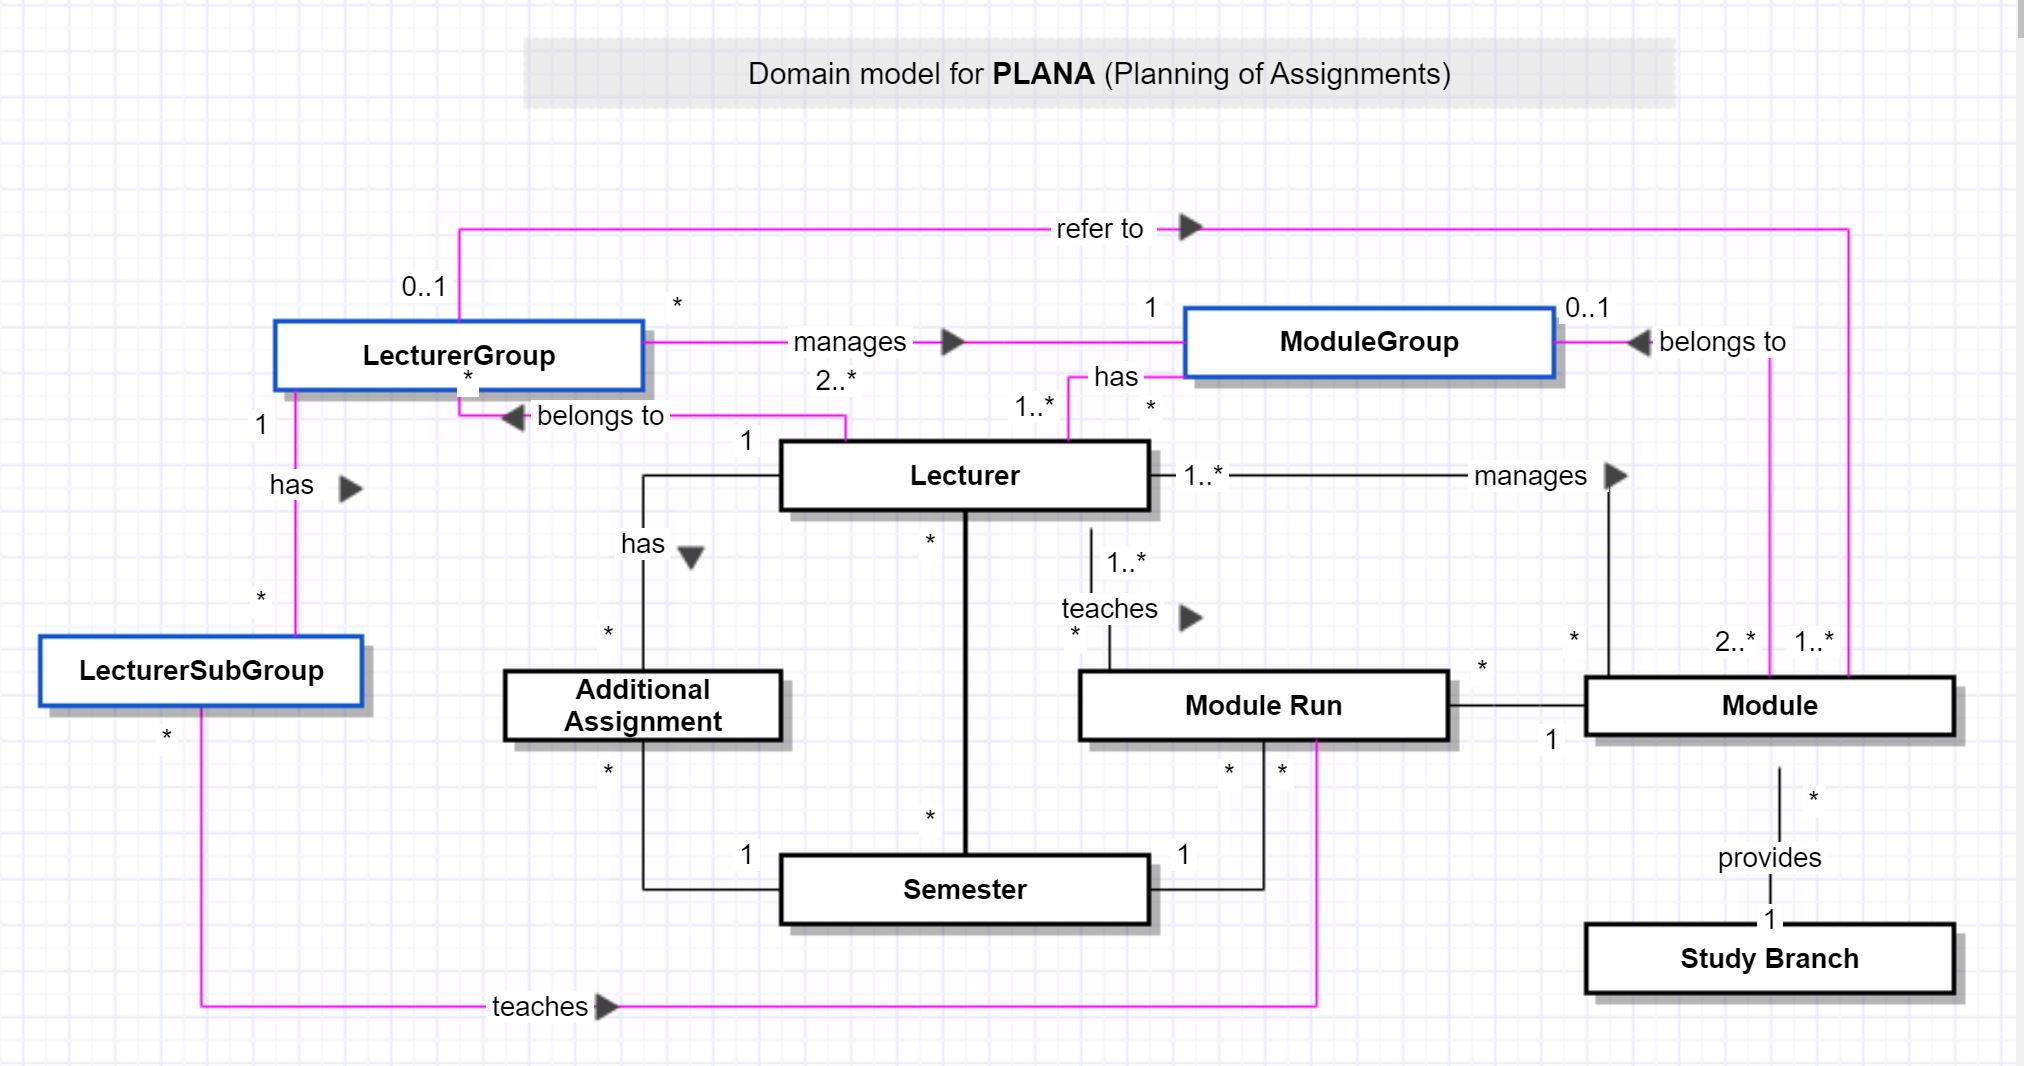
\includegraphics[width=150mm]{uml/domain-b.JPG}
\caption{Domain Model for PLANA}
\label{blabla}
\end{figure}

In the domain model (Figure 2) we added small changes.
When analyzing graphic concepts and the domain model, we found that it is necessary to add associations between the teacher and the teacher subgroup, since they are directly related. 


\begin{figure}[H]
\centering
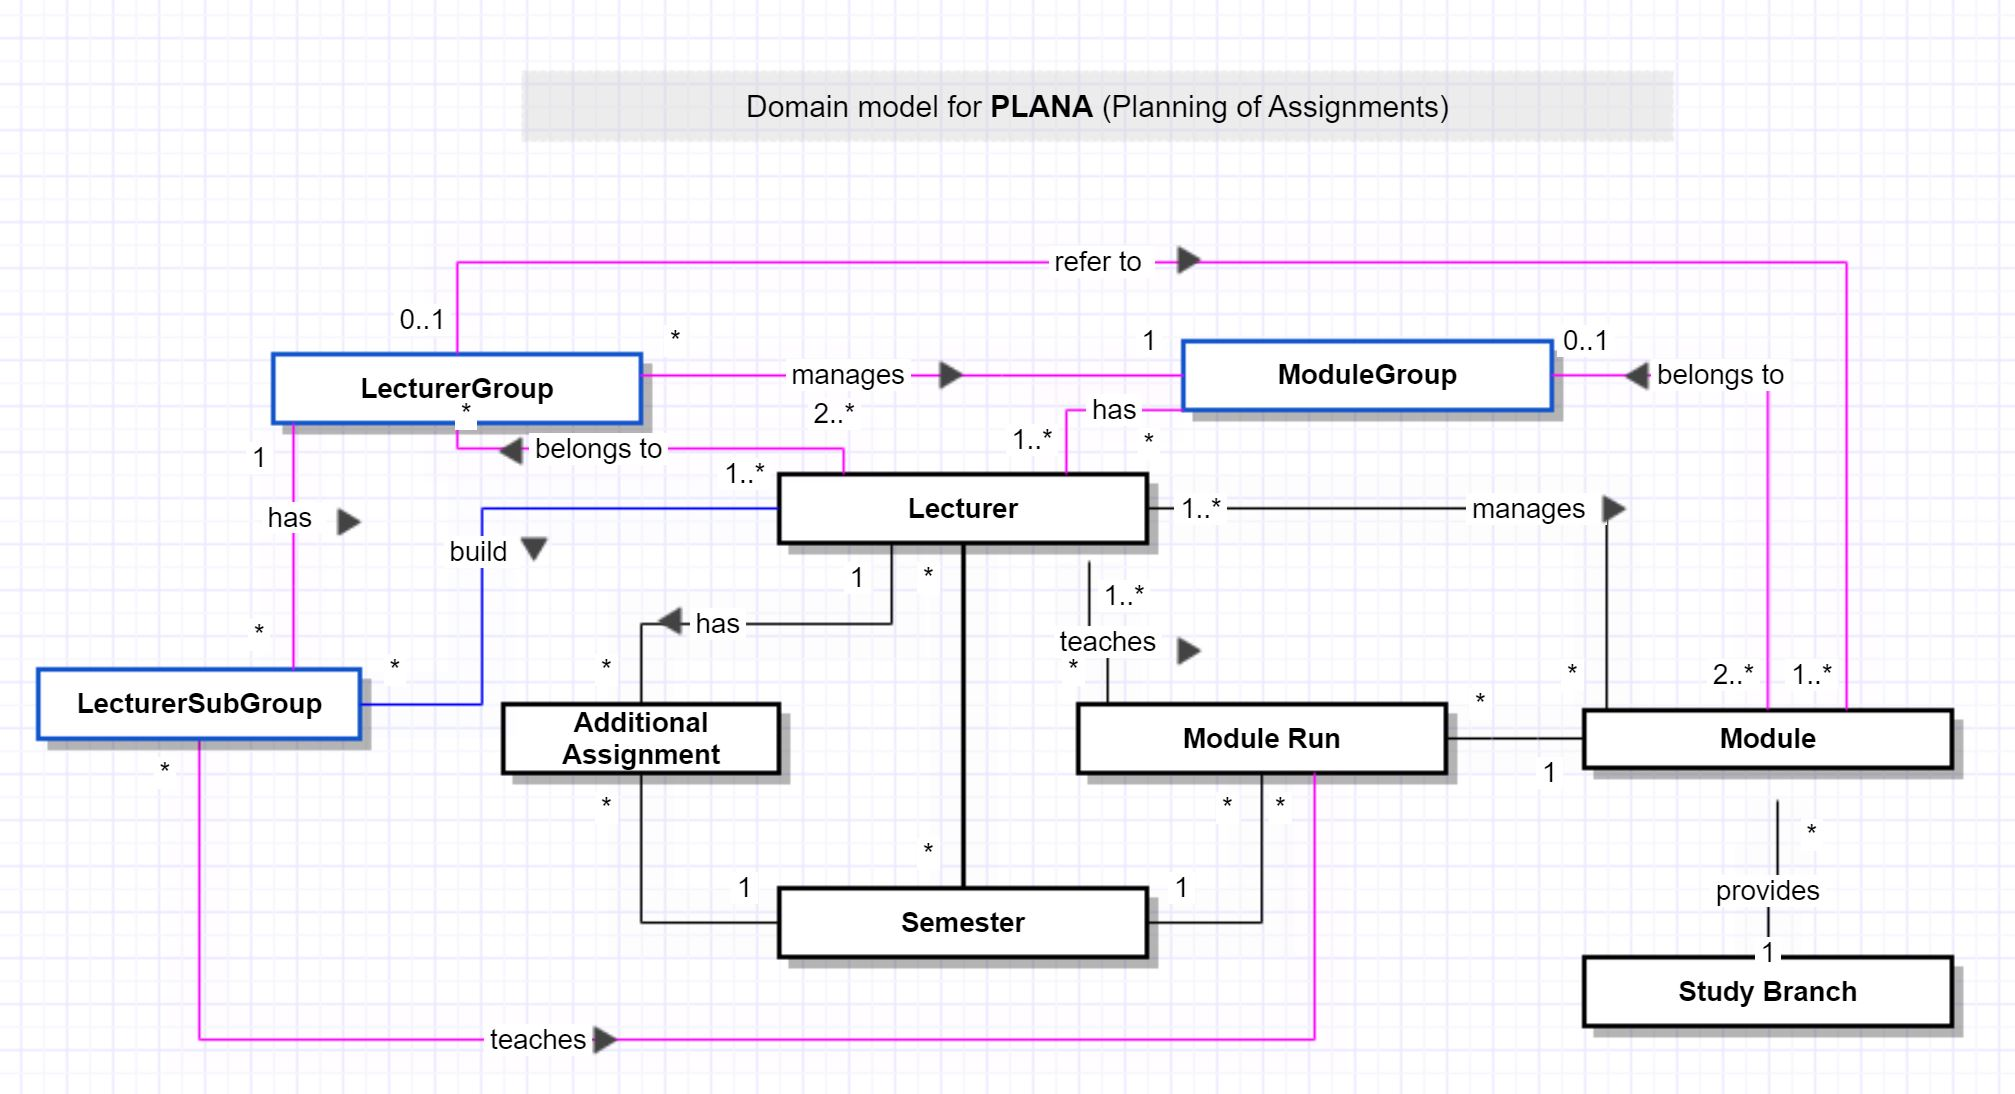
\includegraphics[width=150mm]{uml/domain-b2.JPG}
\caption{Domain Model for PLANA}
\label{blabla}
\end{figure}


The domain model (Figure 3) is the post-analysis Domain model. We have removed the LecturerSubGroups, as we decided that they would not be useful to us. And also, we removed the links between the Module and Module Group and added it between the Module Run and the Module Group, since it is intended to create a groups of the Module Runs.
\begin{figure}[H]
\centering
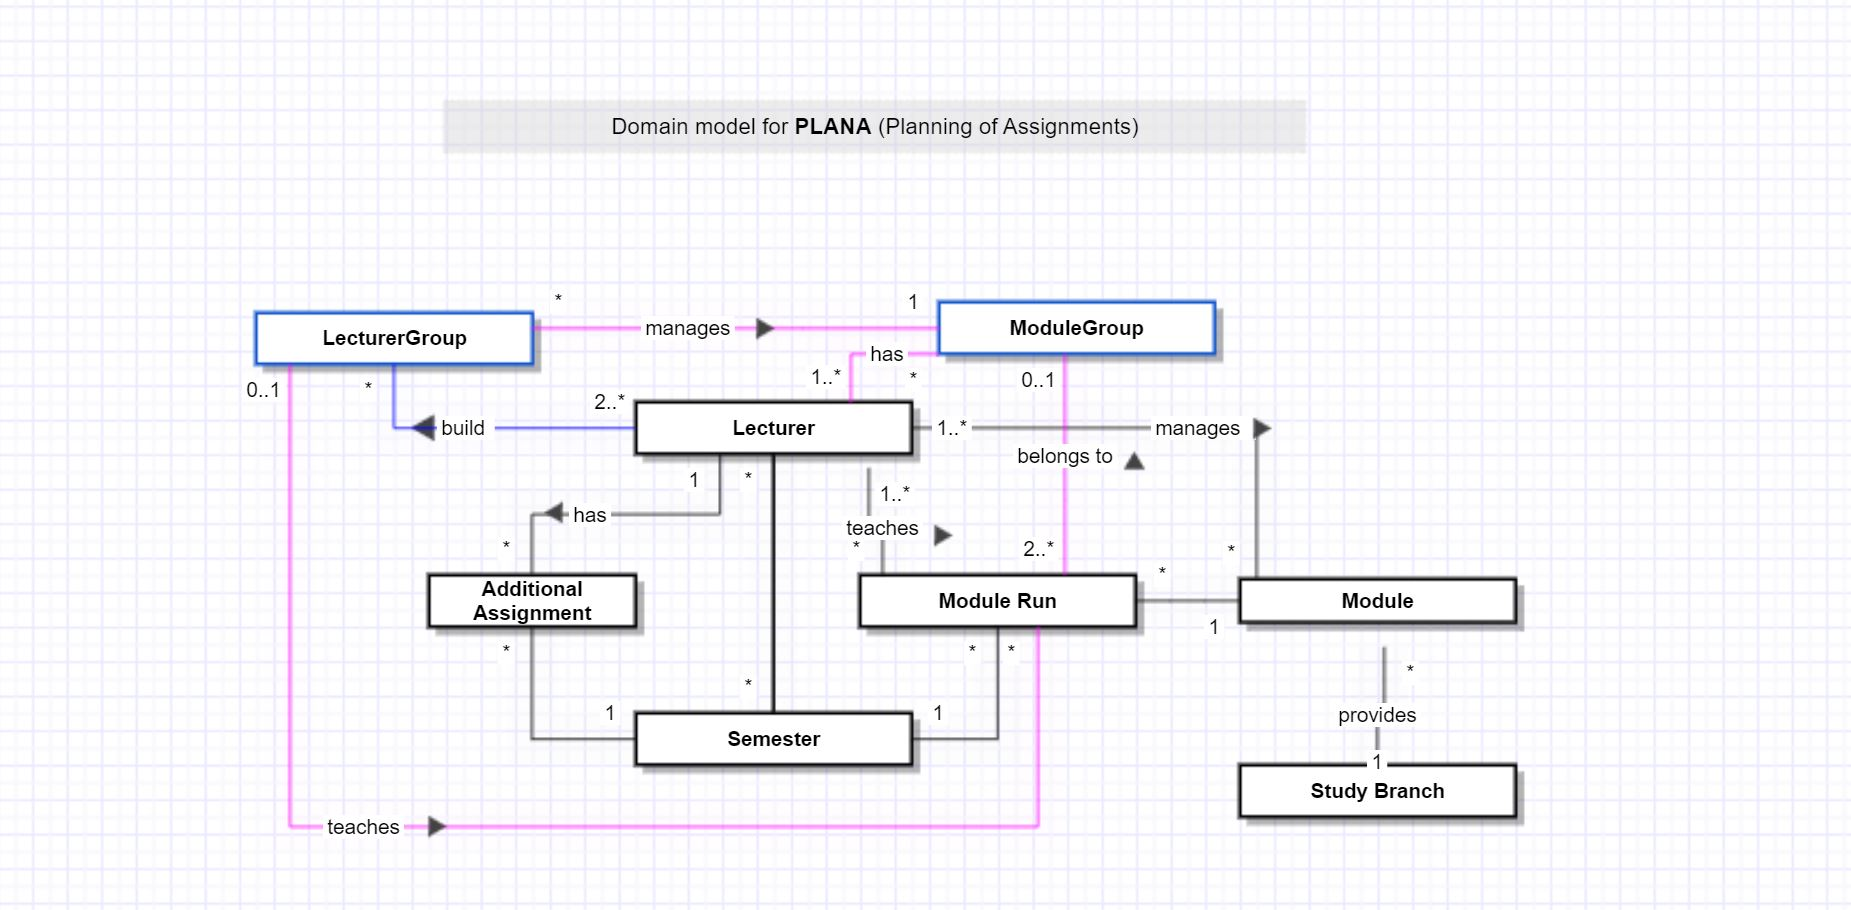
\includegraphics[width=150mm]{uml/domain-b3.JPG}
\caption{Domain Model for PLANA}
\label{blabla}
\end{figure}

In the definition of concepts, new concepts, associations between them and other concepts are highlighted in blue.

	    \subsubsection{i. Concept Definition}
	    
	    \begin{itemize}
	    \item Concept class \textbf{Lecturer} models a person who teaches in a school.
	     \item Concept class \textbf{Study Branch} models a conceptual subdivision of subjects that form a study programme.
	      \item Concept class \textbf{Module} models a set of independent units that form a course at the school.
	       \item Concept class \textbf{Module Run } models executions of a course in different languages.
	       	      \item Concept class \textbf{Additional Assignment} models a set of independent units that form an additional task for the assignment's plan for the lecturer.
  \item Concept class \textbf{Semester} models the periods in the year, during which the lecturer is present in the school.
  \item Concept class \textbf{\textcolor{blue}{ LecturerGroup}} models   group of teachers who will jointly participate in one or more modules.
   \item Concept class \textbf{\textcolor{blue}{ModuleGroup }}  models
   several modules collected in groups for further effective use.
     \item Concept class \textbf{\textcolor{blue}{LecturerSubGroup }} models subdivision of the main group of teachers to carry out the module in different student groups.
     
	         
	    \end{itemize}


 \subsubsection{ii. Association Definition}
	    \begin{table}[H]
\begin{center}
\begin{tabular}{| p{6.5cm}| p{6.5cm} |p{2.5cm}|}

\hline
\rowcolor{LightCyan}
\textbf{Concept Pair} & \textbf{Association Definition}& \textbf{Association Name} \\
\hline
Lecturer -> Module Run                    &    Lecturer can teach zero or        more Module Runs . Each Module Run can be taught by  one or more Lecturers 	& teaches\\ \hline

Semester -> Module Run                    &      Semester can include zero or more Module Runs  .    	& includes\\ \hline

Semester -> Additional Assignment     &     Semester can include zero or more Additional Assignments      & includes\\ \hline

Lecturer -> Additional Assignment                    &    Lecturer can have zero or more Additional Assignments 	& has\\ \hline

Lecturer -> Module                    &             Lecturer can manage zero or more Modules. A module can be managed by one or more Lecturers	& manages\\ \hline

Module -> Module Run                    &    Module is executed as many
as there are module runs or not executed at all.
A Module run is executed for one Module.& executes \\ \hline

Study Branch -> Module                    &   Each Study Branch has many modules. These modules belong to exactly one study branch.  & has\\ \hline
  Semester -> Lecturer                  &      In each Semester, there are many lecturers that are teaching, and these teachers are teaching in more than one Semester       & includes\\ \hline
 

 
\textbf{\textcolor{blue}{ LecturerGroup -> Module}}  & 
 Each Module can have maximal one LecturerGroup. LecturerGroup can refer to multiple Modules. &  refer to\\ \hline
 
 \textbf{\textcolor{blue}{ Lecturer -> LecturerGroup}}  & 
 Each Lecturer can belongs to zero or more group. 
 Each LecturerGroup must consist of two or more lecturers. &  belongs to\\ \hline
 
  \textbf{\textcolor{blue}{  LecturerGroup -> LecturerSubGroup}}  & 
 Each LecturerGroup can have from zero to many LecturerSubGroups.
 LecturerSubGroup can refer to exactly one LecturerGroup &  has\\ \hline
 
\textbf{\textcolor{blue}{LecturerSubGroup -> ModuleRun}}  &  Each LecturerSubGroup can teach zero to many Module Run.A Module Run can be taught by zero or several LecturerSubGroup.
 & teaches\\ \hline

\textbf{\textcolor{blue}{Module -> ModuleGroup}}  &  
A Module can belong to zero or one ModuleGroup. ModuleGroup can have from two to many Modules. & belongs to\\ \hline

\textbf{\textcolor{blue}{LecturerGroup -> ModuleGroup}}  &  A LecturerGroup can manage exactly one ModuleGroup. A ModuleGroup can have zero to many LecturerGroup.
. & manages\\ \hline

\textbf{\textcolor{blue}{Lecturer -> LecturerSubGroup}}  &  Lecturers can build zero or many LecturerSubGroups. LecturerSubGroup can contain from one to many Lecturers in it.
. & build\\ \hline
\end{tabular}
\end{center}
\caption{Association Definition}
\label{table2}
\end{table}


\section{Technologies}

%%%implementation
\section{Creating the Projects}

\subsection{Structure of Projects and Folders}

\subsection{Data Models}

\subsection{Entity Framework Core Packages}

\subsection{Connection String}

\subsection{Creating the Database Context Class}

\subsection{Entity Framework Core Configuration}

\subsection{Database and Entity Framework Core}
Entity Framework(EF) Core is an object-relational mapper (O /RM). It is designed to make writing code for accessing a database quick and intuitive.
There are many good reasons to use EF Core. It supports LINQ queries, change tracking, updates, and schema migrations. EF Core works with many databases, including SQL Database, SQLite, MySQL, PostgreSQL, and Azure Cosmos DB.
book \cite{efa} \cite{ef}

\subsection{The PLANA App's Relational Database}
Our database has many types of relationships we can have in EF Core. The types are:
One-to-many: Lecturer
Many-to-many:
One-To-Many Relationship : 
Lecturer to an Additional Assignment 
Semester to a Additional Assignment
Semester to a Module Run 
Module to a Module Run
Study Branch to a Module
Many-To-Many Relationship :
Lecturers to Semester
Lecturers to Module
Lecturers to Module Run




\subsection{Modeling Types of Database Relationships}
\subsubsection{Many-to-many Relationship }
Creating many-to-many relationship is little bit different from the one-to-many and one-to-one.
We will take as example relation between Lecturer and Module.\\

In EF Core database doesn't directly implement this kind of relationships.
First we have to create class Lecturer and class Module. Then we have to create one more class, we call it LecturersModules. This class links lecturers to their modules. \\
At the LecturerModules class there are two properties, LecturerId and ModuleId. There are both - primary keys and foreign keys, known as a composite key.\cite{efa}


\begin{figure}[H]
\centering
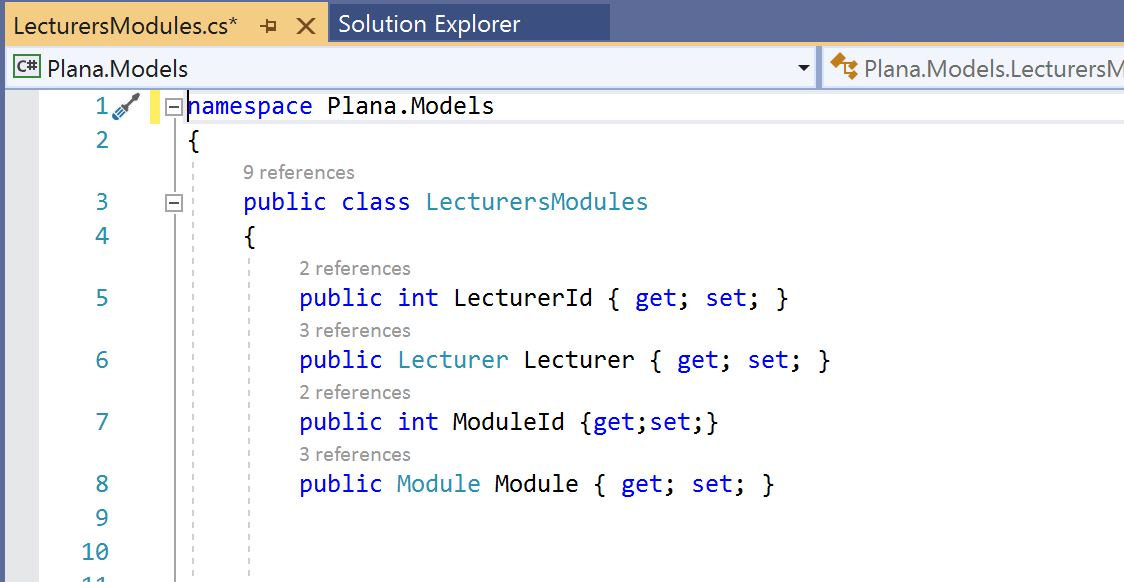
\includegraphics[width=150mm]{report_img/lecturers-modules.JPG}
\caption{The LecturersModules entity class}
\label{blabla}
\end{figure}

 The next step  is adding necessary code to the AppDbContext class. We add 
 \begin{itemize}
 \item \textbf{DbSet<Lecturer>} 
 \item \textbf {DbSet<Module>}
 \item \textbf{DbSet<LecturersModules>}
 \end{itemize}
 
 
 
The Figure 2 below shows this process. In the OnModelCreating method we add
\begin{itemize}
\item\textbf{modelBuilder.Entity<LectuerersModules>().HasKey(x=> new {x.LecturerId, x.ModuleId}};
\end{itemize}


 





\begin{figure}[H]
\centering
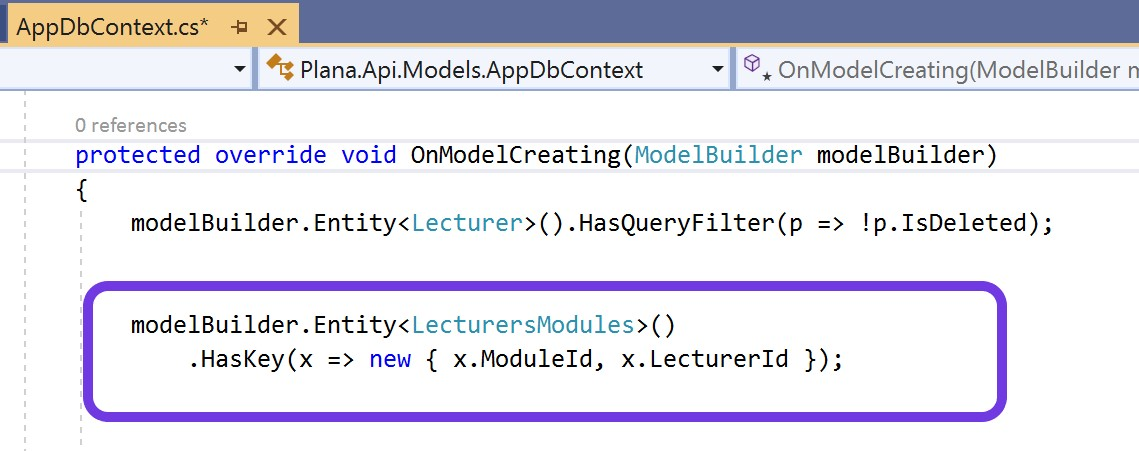
\includegraphics[width=150mm]{report_img/many-to-many.JPG}
\caption{Adding Entity LecturersModules to the AppDbContext class}
\label{blabla}
\end{figure}  
We need write just this and Entity Framework Core will do the correct implementation that we can see then in the migration files. \cite{patrick}

\begin{figure}[H]
\centering
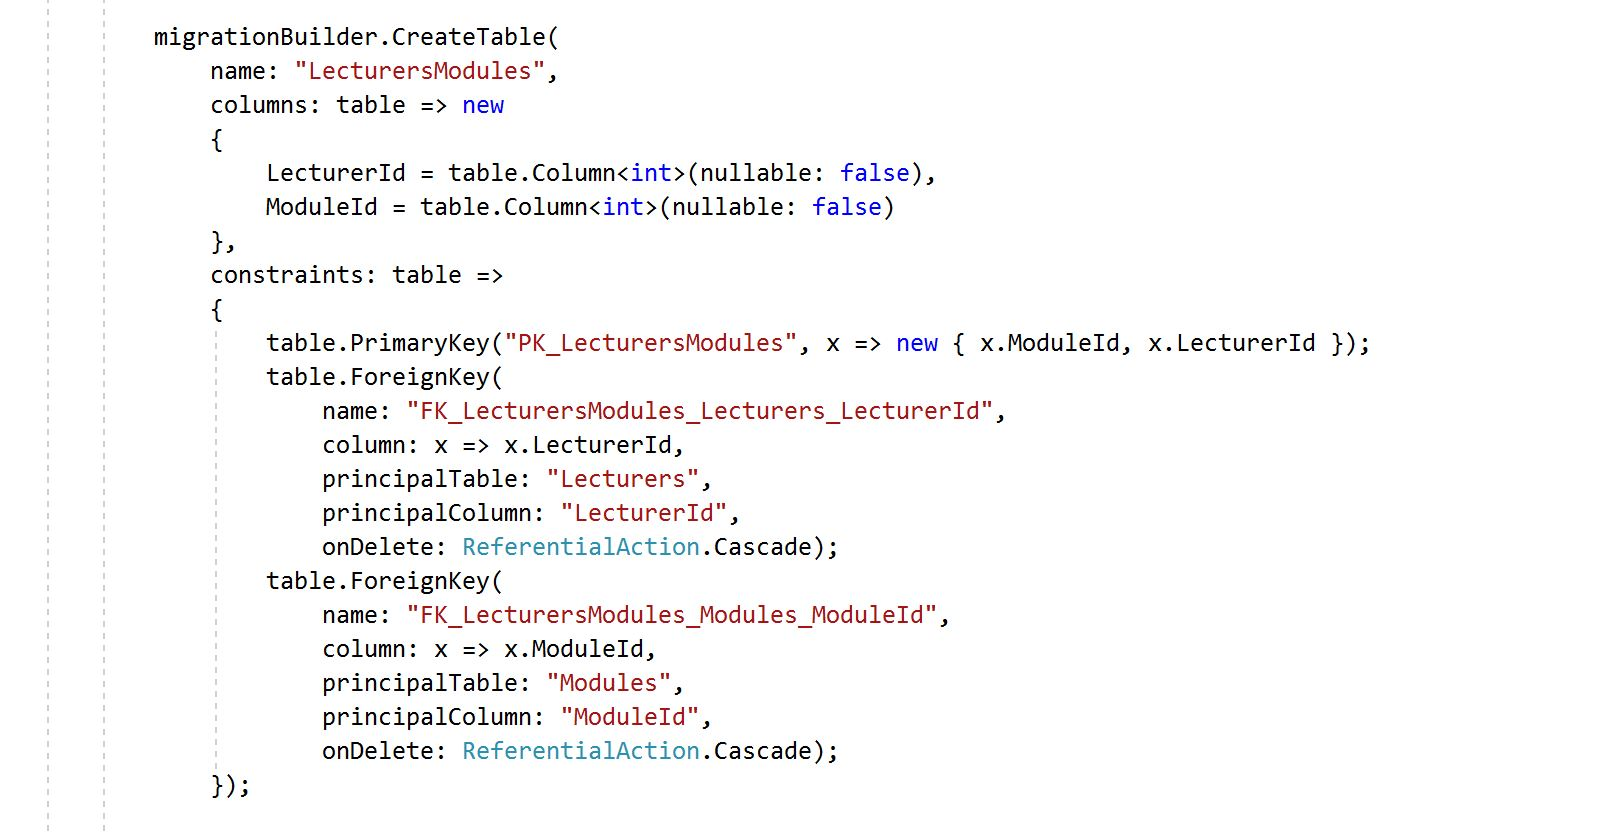
\includegraphics[width=150mm]{report_img/Initial.JPG}
\caption{Initial Migration File}
\label{blabla}
\end{figure} 

From Figure 3 we can see that one many-to-many relationship has transformed in two one-to-many and many-to-one relationships.

\begin{figure}[H]
\centering
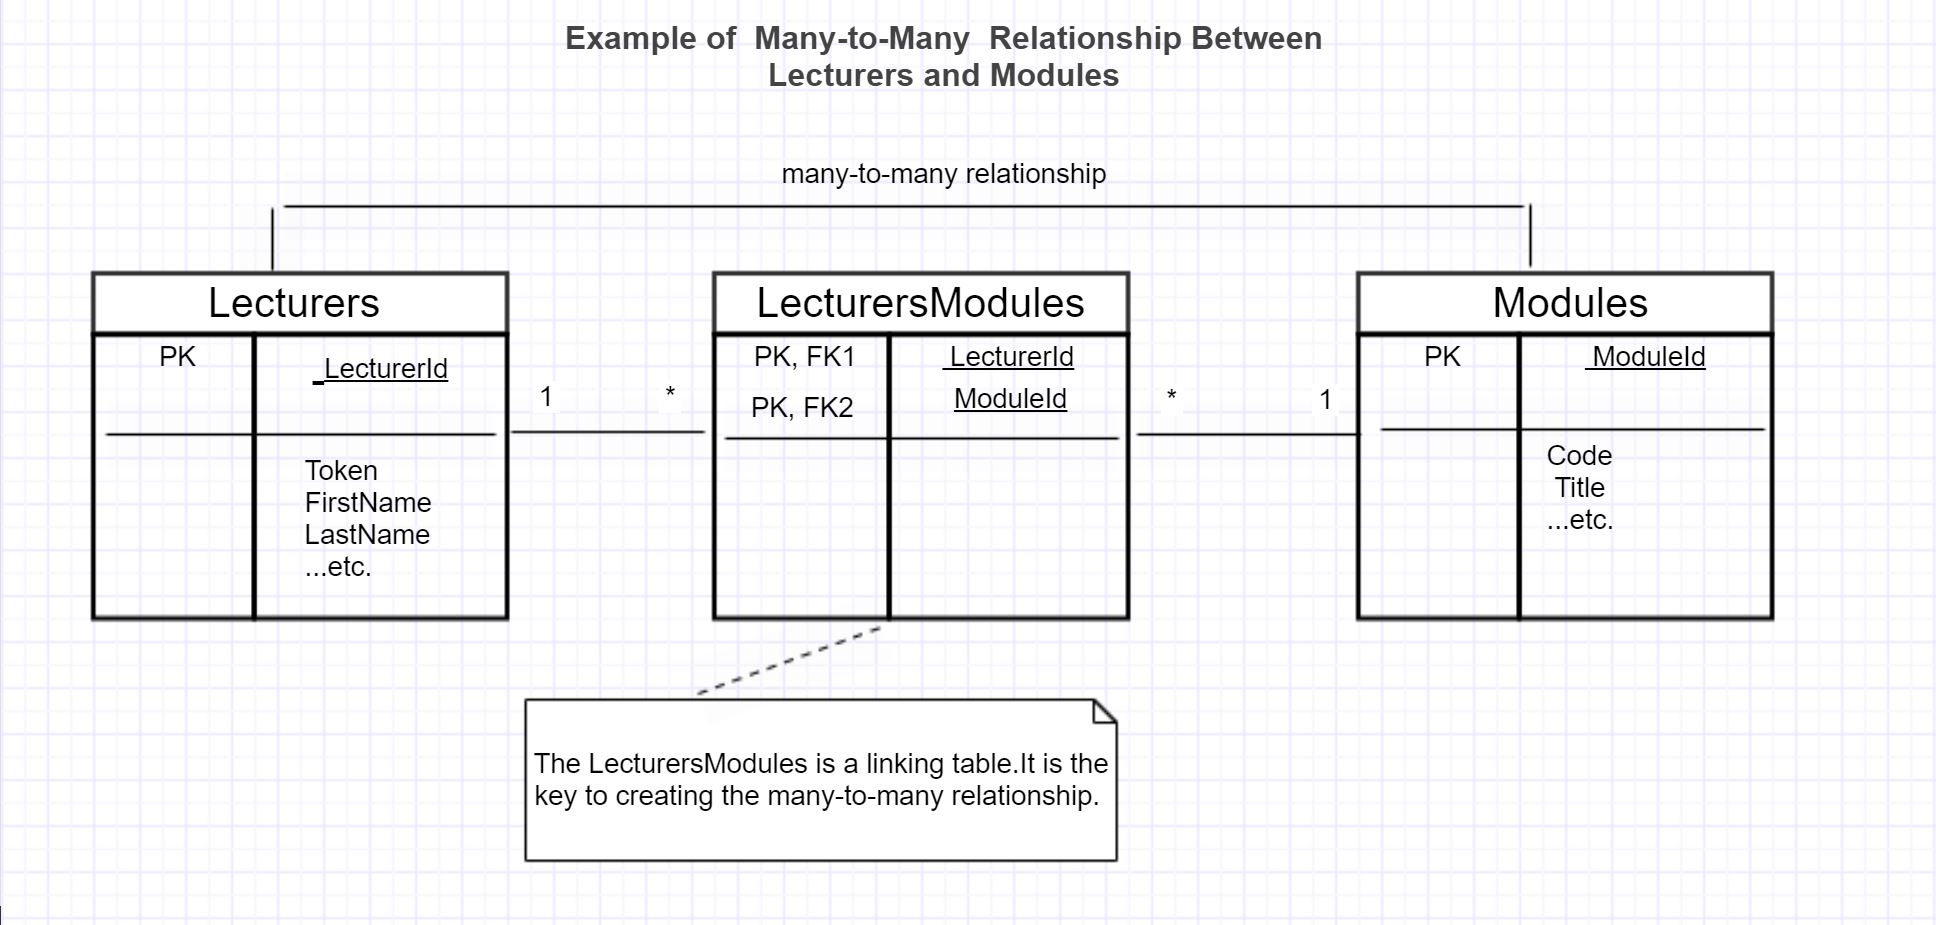
\includegraphics[width=150mm]{report_img/many-to-many-tables.JPG}
\caption{Creating Many-To-Many Relationship}
\label{blabla}
\end{figure}



\subsection{Creating Database}
\newpage
\subsection{Creating a Repository}

todo: photo of repository



In our project we create a repository interfaces and implementation classes.\\
We use \textbf{IQueryable<T> and IEnumarable<T>} interfaces.
With IQueryable<T> interface the objects can be queried in more efficient way.\\
For example: \textbf{public IQueryable<ModuleRun> ModuleRuns => appDbContext.ModuleRuns;} the ModuleRuns property in the context class returns a DbSet<ModuleRun> object, which implements the IQueryable<T> interface.

\noindent                                                                %
\begin{minipage}{\linewidth}                     
\makebox[\linewidth]{                                      
  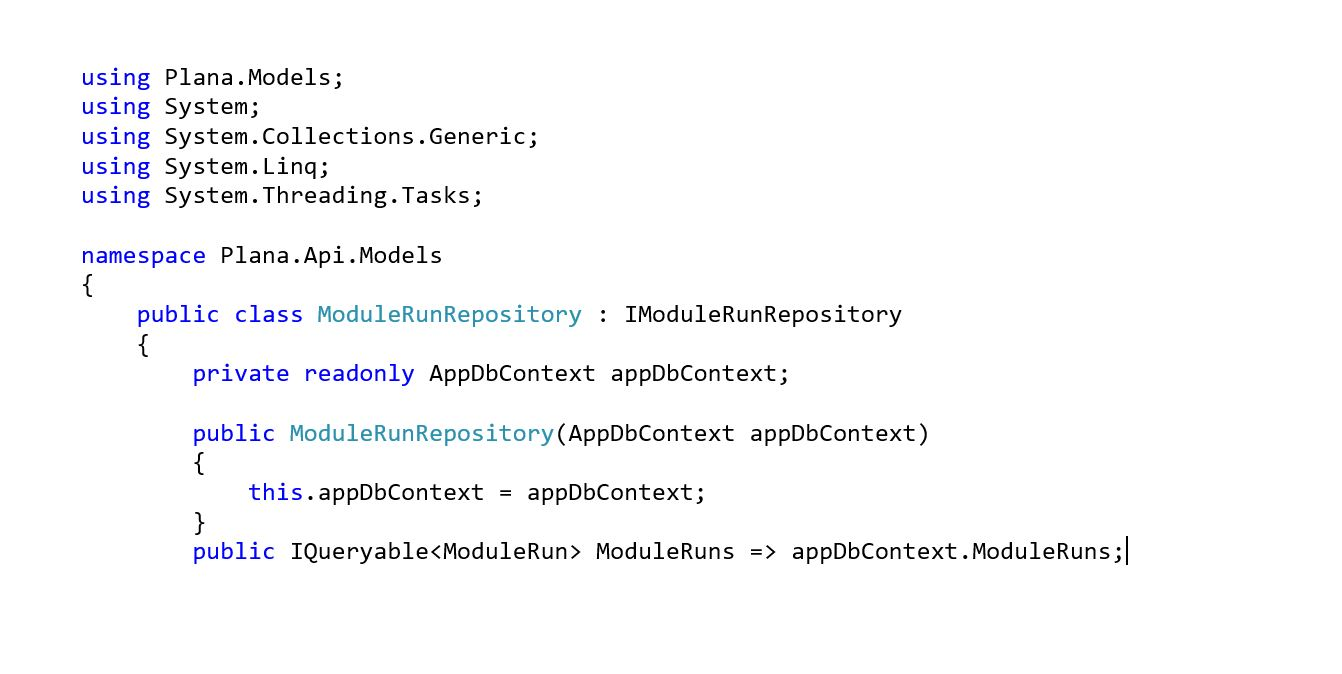
\includegraphics[keepaspectratio=true,scale=0.9]{report_img/repo-create.JPG}}
\captionof{figure}{The ModuleRunRepository.cs file in the Plana.Api/Models folder}
%\label{visina8                                                      }%  only if needed  
\end{minipage}


\newpage

Then we create the Repository Service in the Startup.cs file.\\

\begin{figure}[h]
\centering
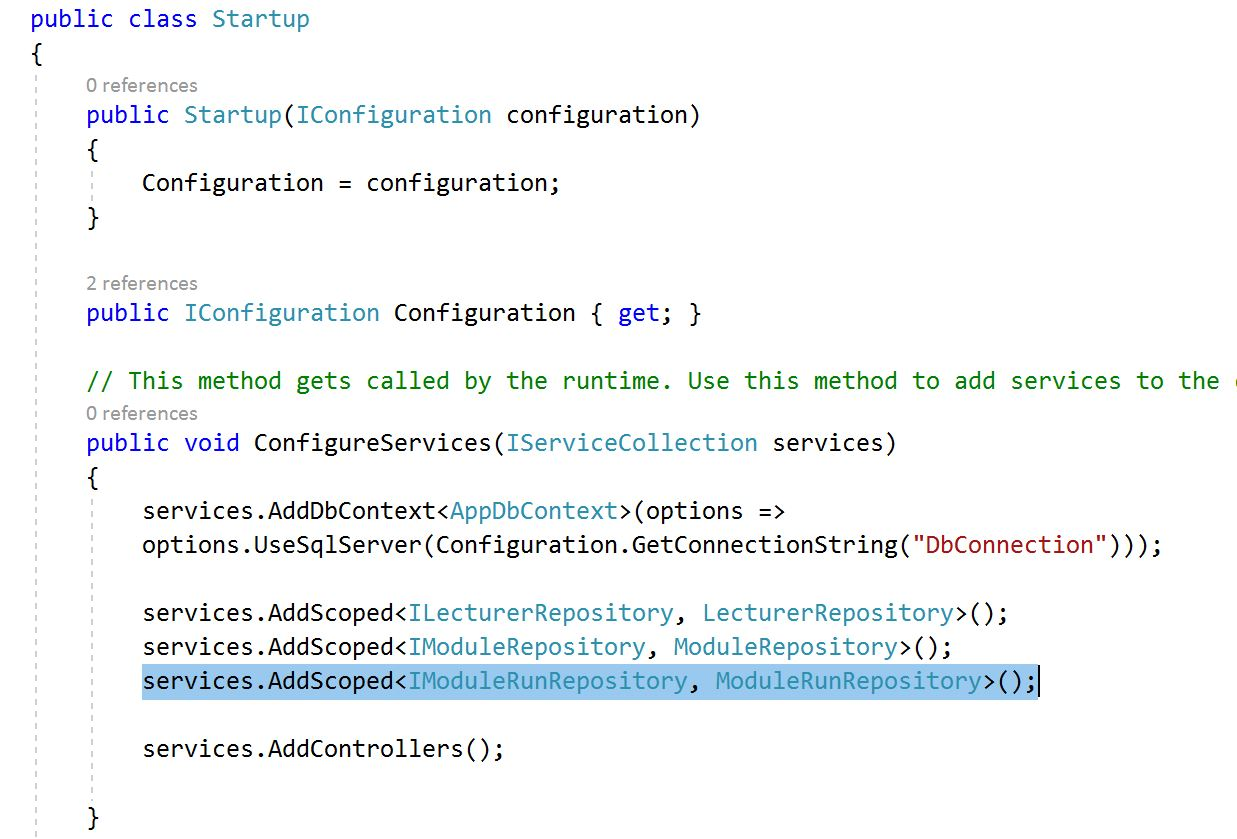
\includegraphics[width=150mm]{report_img/add_scoped_rep.JPG}
\caption{Creating Services in Startup.cs File}
\label{blabla}
\end{figure}

 

\cite{core3}

\subsubsection{Creating the Database Migration, Code-First Migration}
Entity Framework Core makes it possible to generate schema for the database from the data model classes using \textbf{migrations}
\textbf{dotnet em migrations add Initial} 
\cite{core3}



\subsection{Creating Seed Data}
The seed data is the data that is used to populate the database. For seed data we add class SeedData.cs in the Models folder in Plana.Api project \cite{core3}.
%\subsubsection{Delete method in Entity Framework Core}
By default, Entity Framework Core uses cascade deletes for depend relationships with non-nullable foreign keys. \cite{efa} \\
..add photo of seed class (give it name The contents of the SeedData.cs class \\
\subsubsection{Configuration of Core Services and Entity Framework}

It is necessary to make changes in Startup.cs class in Plana.Api project - configure Entity Framework Core and set up the services that will be used to access the database \cite{efa}.\\
The figure below shows all these configurations.

\noindent%
\begin{minipage}{\linewidth}% to keep image and caption on one page
\makebox[\linewidth]{%        to center the image
  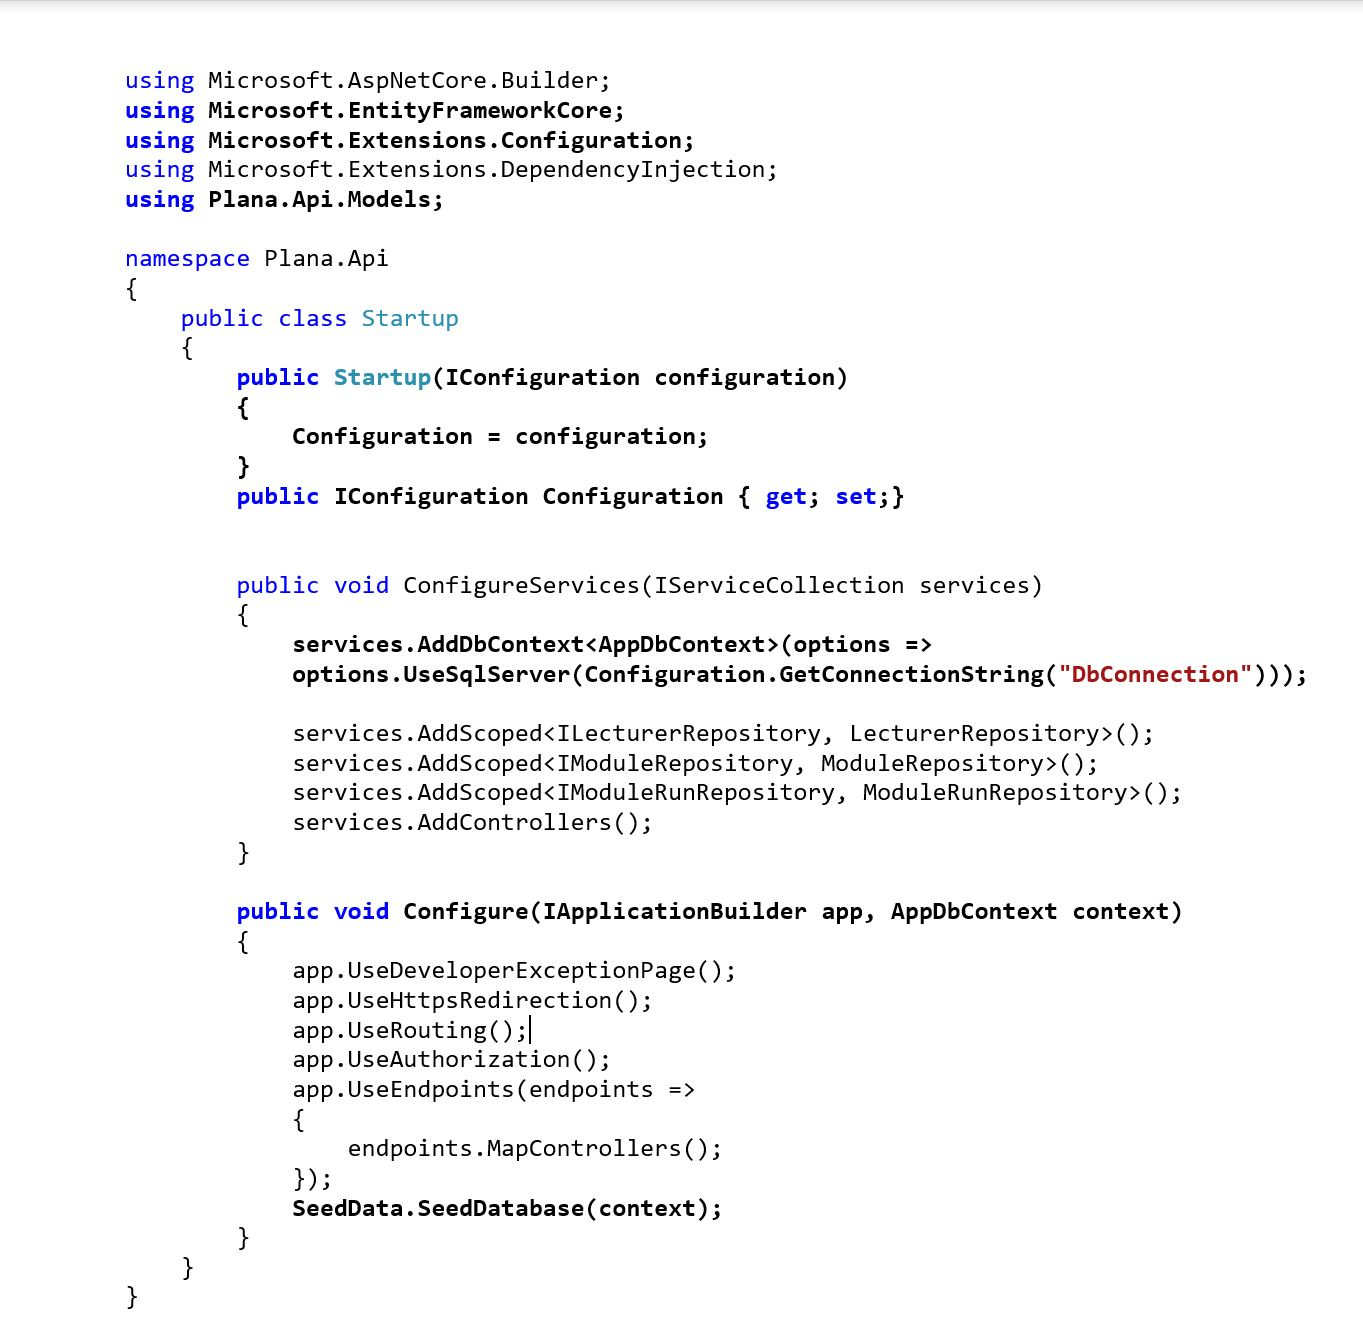
\includegraphics[keepaspectratio=true,scale=0.8]{report_img/seed-data-startup.JPG}}
\captionof{figure}{Startup.cs in the Plana.Api project.Preparing Services and Middleware}
%\label{visina8}%      only if needed  
\end{minipage}


\subsection{Create a Controller}

















%\section{Technologies}


\subsubsection{Complex Data Model}
in this section I would like to highlight more complex features of coding and data model structure in asp .net core.\\

\noindent                                                                %
\begin{minipage}{\linewidth}                            % to keep image and caption on one page
\makebox[\linewidth]{                                       %  to center the image
  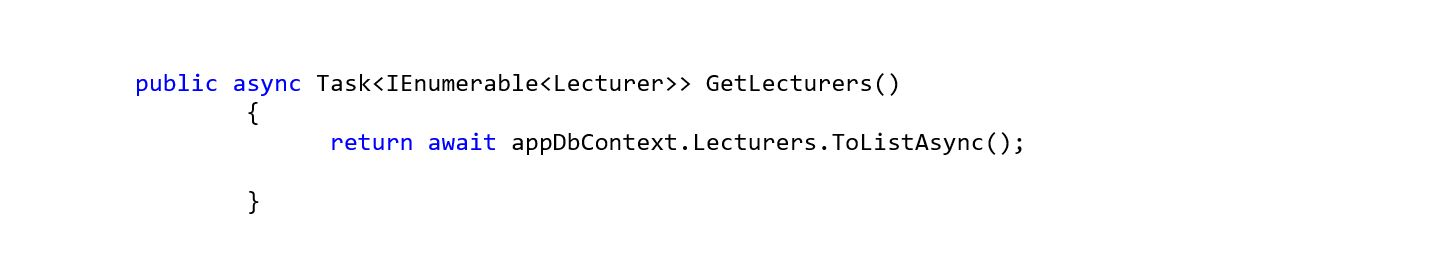
\includegraphics[keepaspectratio=true,scale=0.9]{report_img/complex_data_problem/repository_get_lecturers}}
\captionof{figure}{LecturerRepository.cs file in the Plana.Api project's folder}
\label{visina8                                                      }%  only if needed  
\end{minipage}



\begin{figure}[H]
\centering
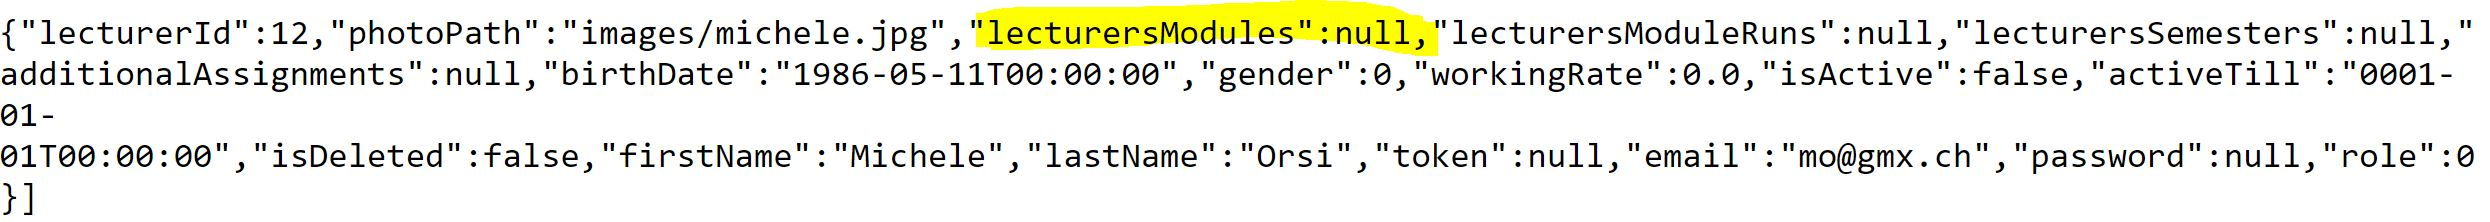
\includegraphics[width=150mm]{report_img/complex_data_problem/michele_module_null}
\caption{}
\label{blabla}
\end{figure}

\noindent                                                                %
\begin{minipage}{\linewidth}                            % to keep image and caption on one page
\makebox[\linewidth]{                                       %  to center the image
  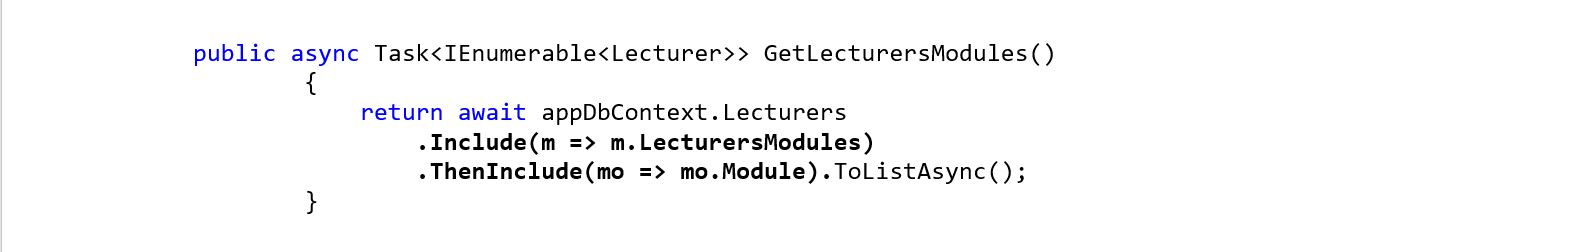
\includegraphics[keepaspectratio=true,scale=0.9]{report_img/complex_data_problem/repository_get_lecturers_modules}}
\captionof{figure}{...}
\label{visina8                                                      }%  only if needed  
\end{minipage}




\begin{figure}[H]
\centering
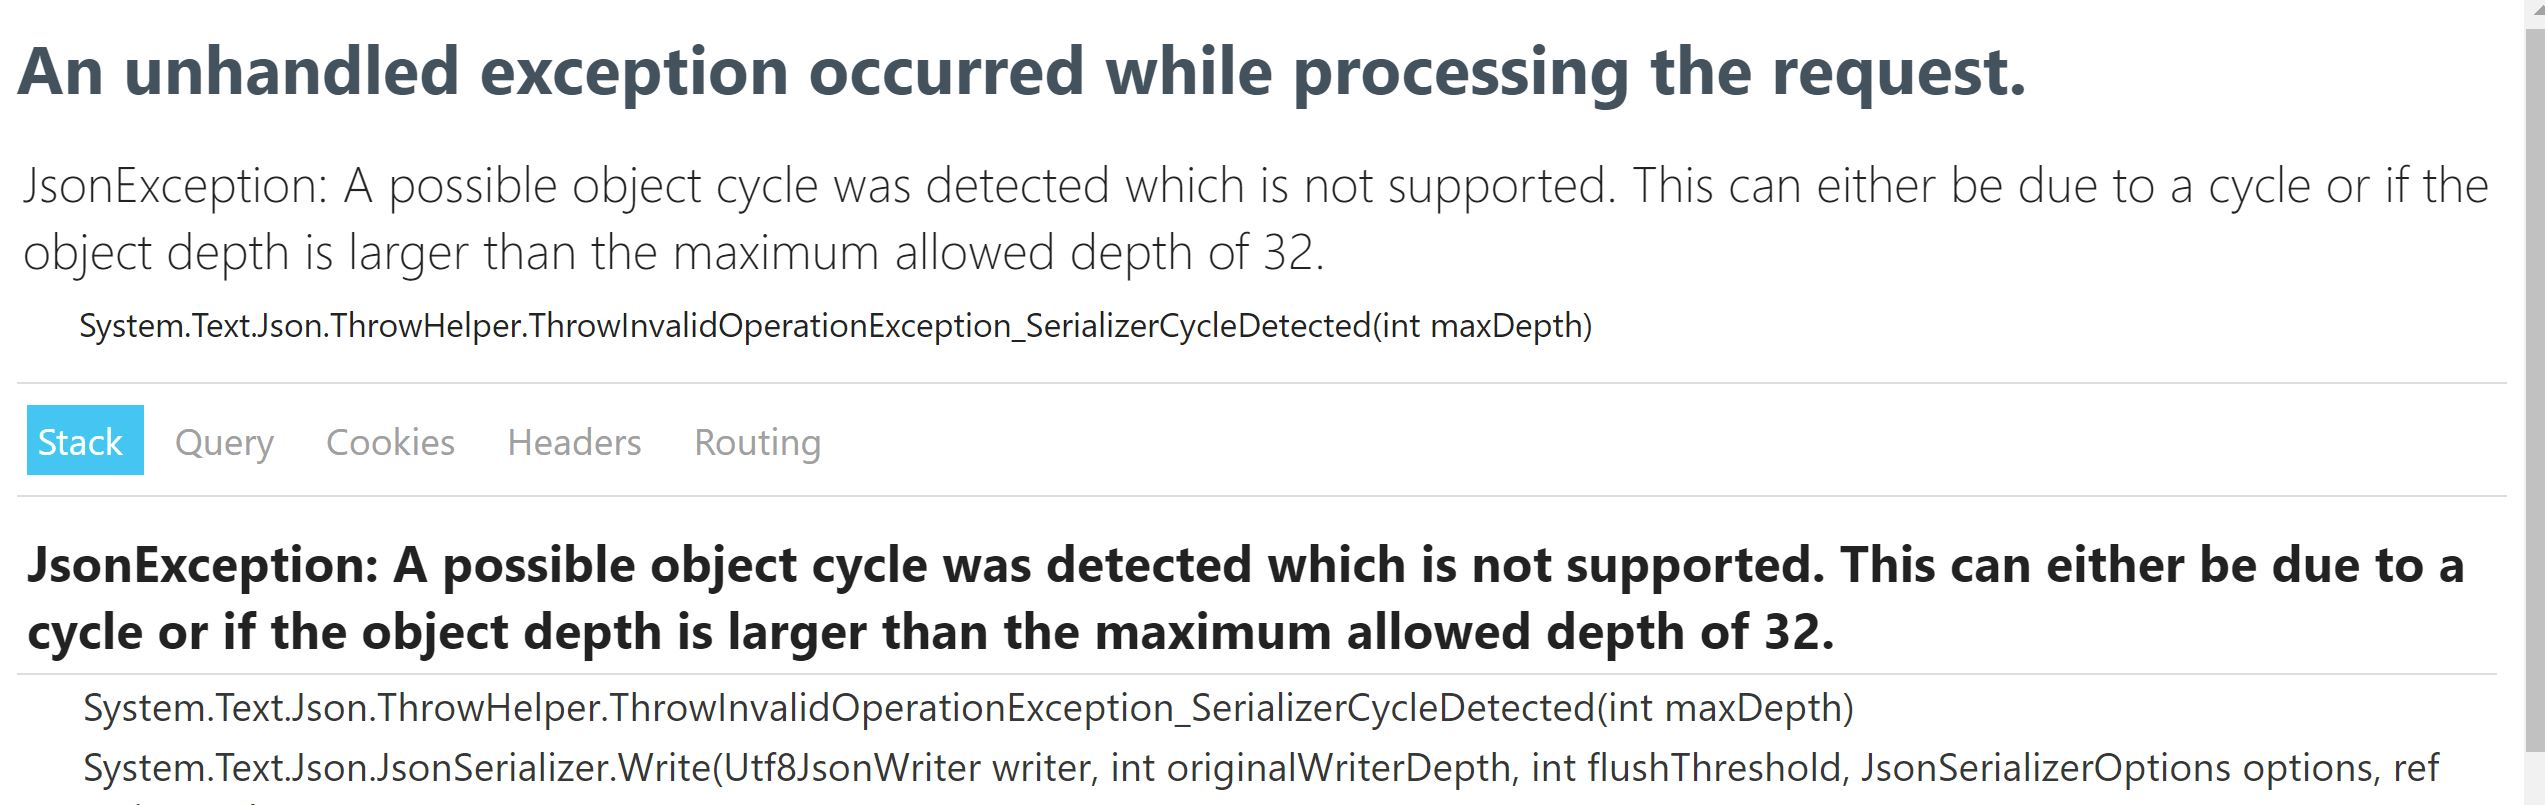
\includegraphics[width=150mm]{report_img/complex_data_problem/json_problem}
\caption{}
\label{blabla}
\end{figure}

\begin{figure}[H]
\centering

\includegraphics[width=150mm]{report_img/complex_data_problem/install_newtonsoft_json}
\caption{}
\label{blabla}
\end{figure}

\noindent                                                                %
\begin{minipage}{\linewidth}                            % to keep image and caption on one page
\makebox[\linewidth]{                                       %  to center the image
  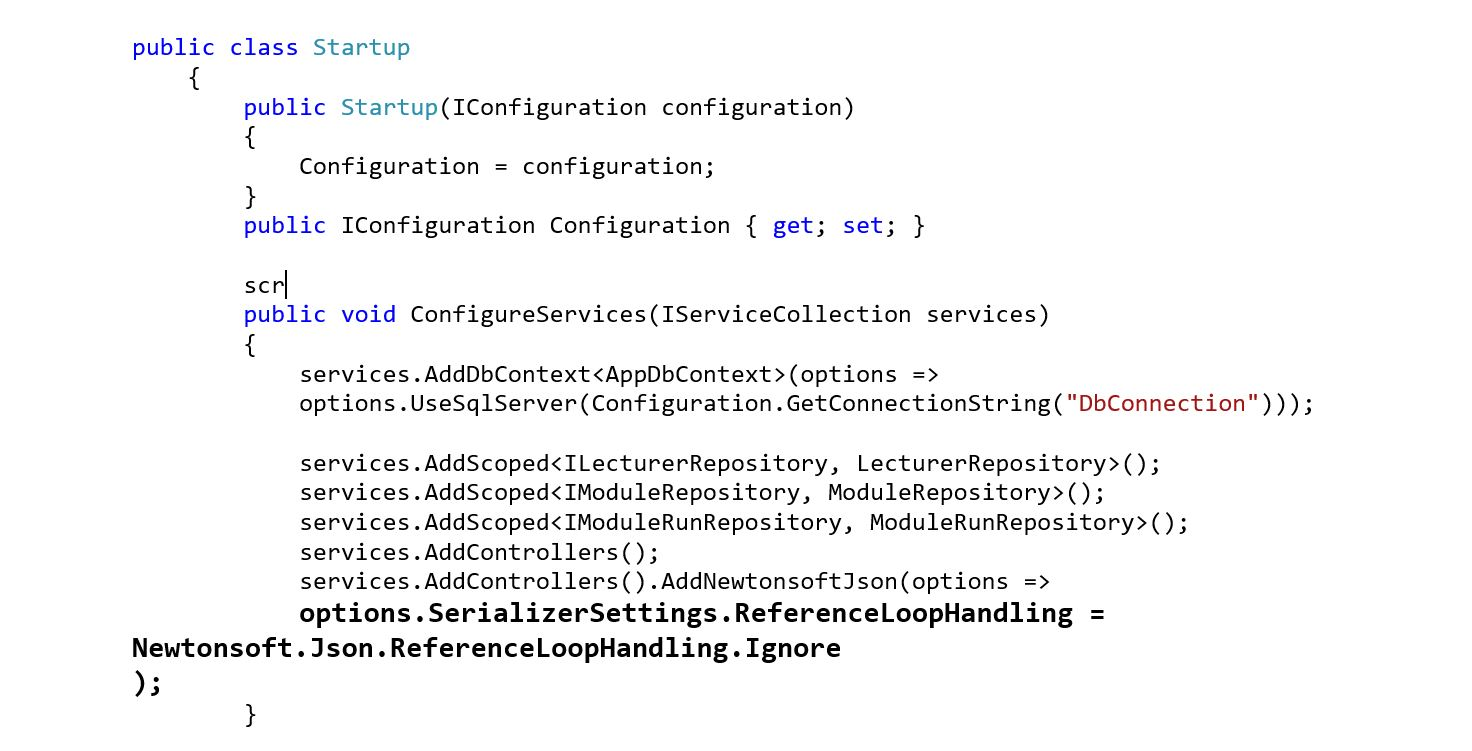
\includegraphics[keepaspectratio=true,scale=0.9]{report_img/complex_data_problem/startup_add_newtonsoft}}
\captionof{figure}{...}
\label{visina8                                                      }%  only if needed  
\end{minipage}




\begin{figure}[H]
\centering
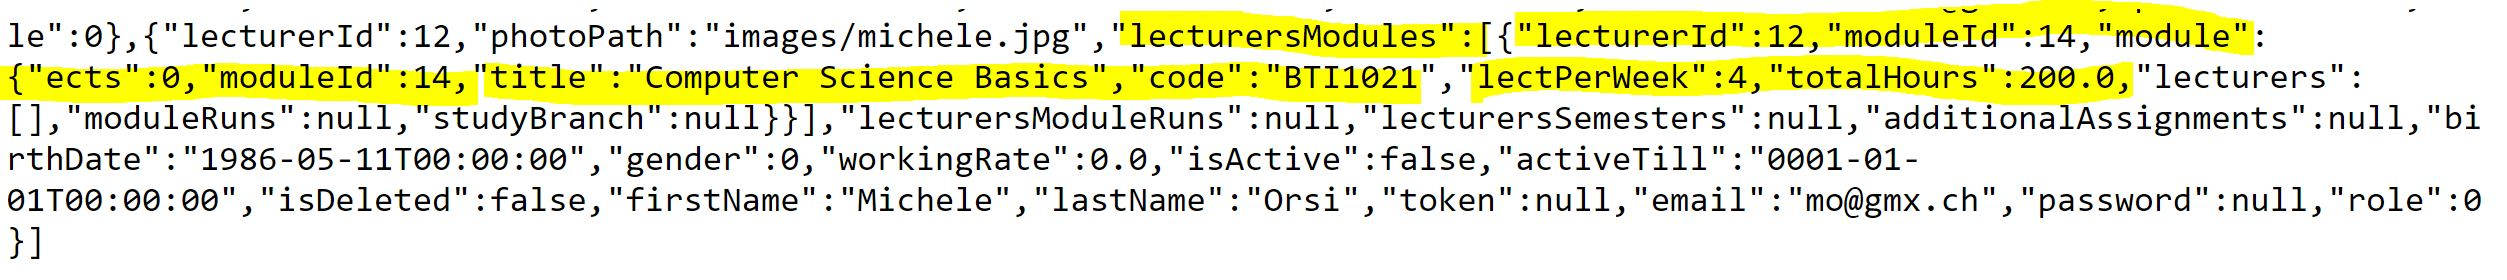
\includegraphics[width=150mm]{report_img/complex_data_problem/michele_module_ok}
\caption{}
\label{blabla}
\end{figure}

\subsubsection{Blazor Server}
\subsubsection{Configuring ASP.NET Core for Blazor Server}

\textbf{Call the API from Asp.net Core Blazor}

.. add picture with a blazor page

...write about imports 

... write about registration of http client services 

\noindent                                                                
\begin{minipage}{\linewidth}                           
\makebox[\linewidth]{                                        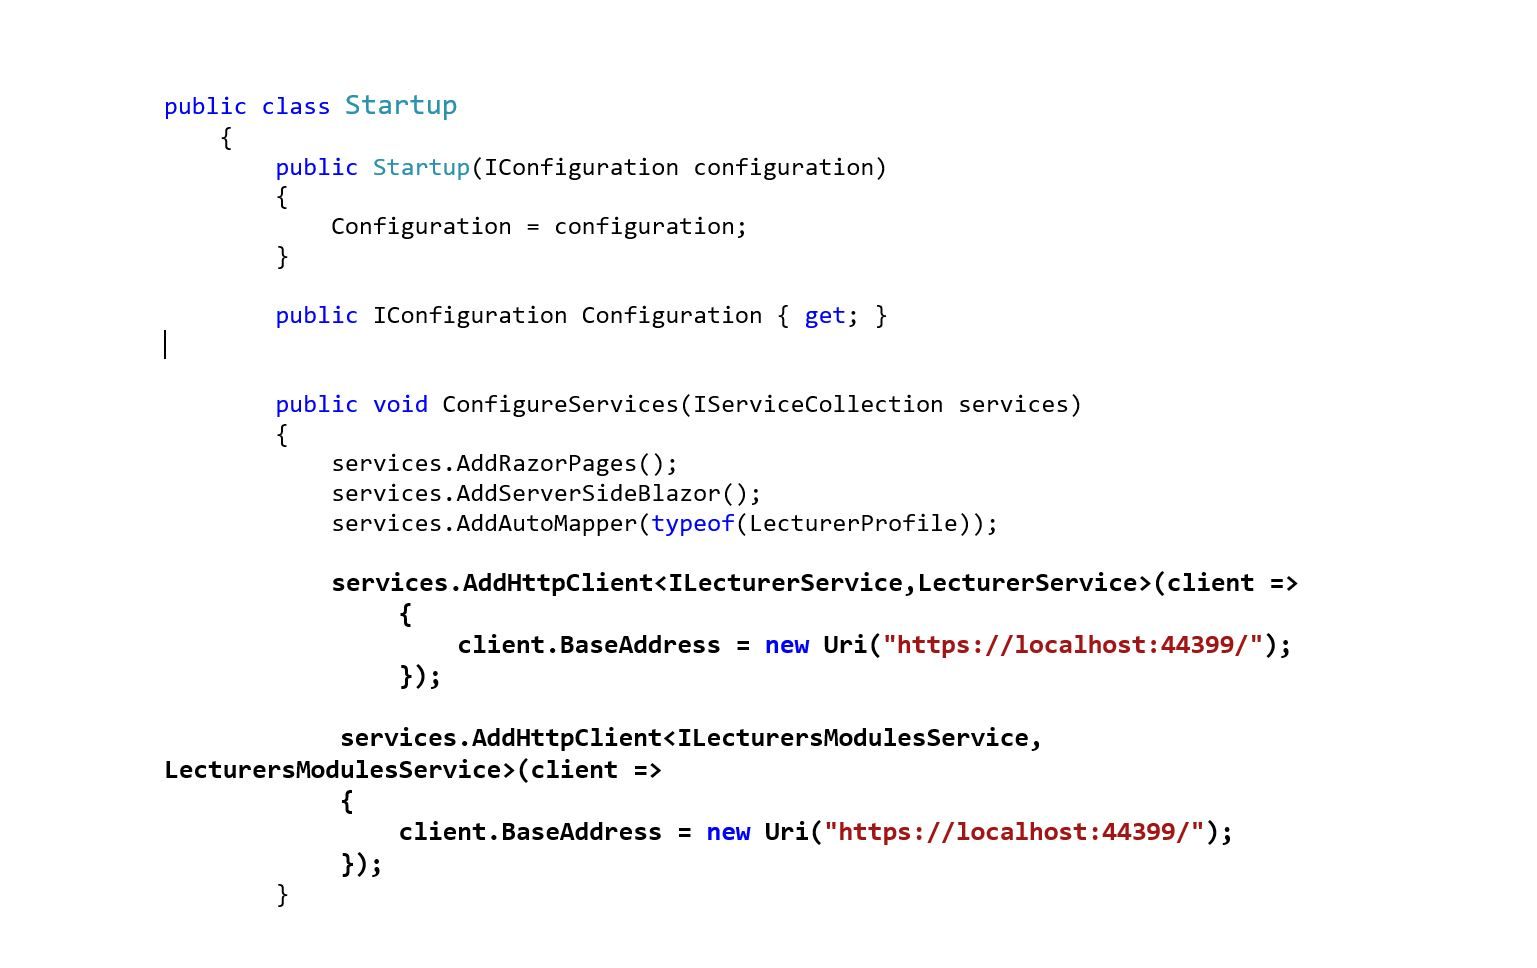
\includegraphics[keepaspectratio=true,scale=0.9]{report_img/blazor/register-http-client}}
\captionof{figure}{Registration of Http Client Services in Startup File in Plana.Web Project folder}
\label{visina8                                                      }
\end{minipage}





\noindent                                                                
\begin{minipage}{\linewidth}                           
\makebox[\linewidth]{                                      
  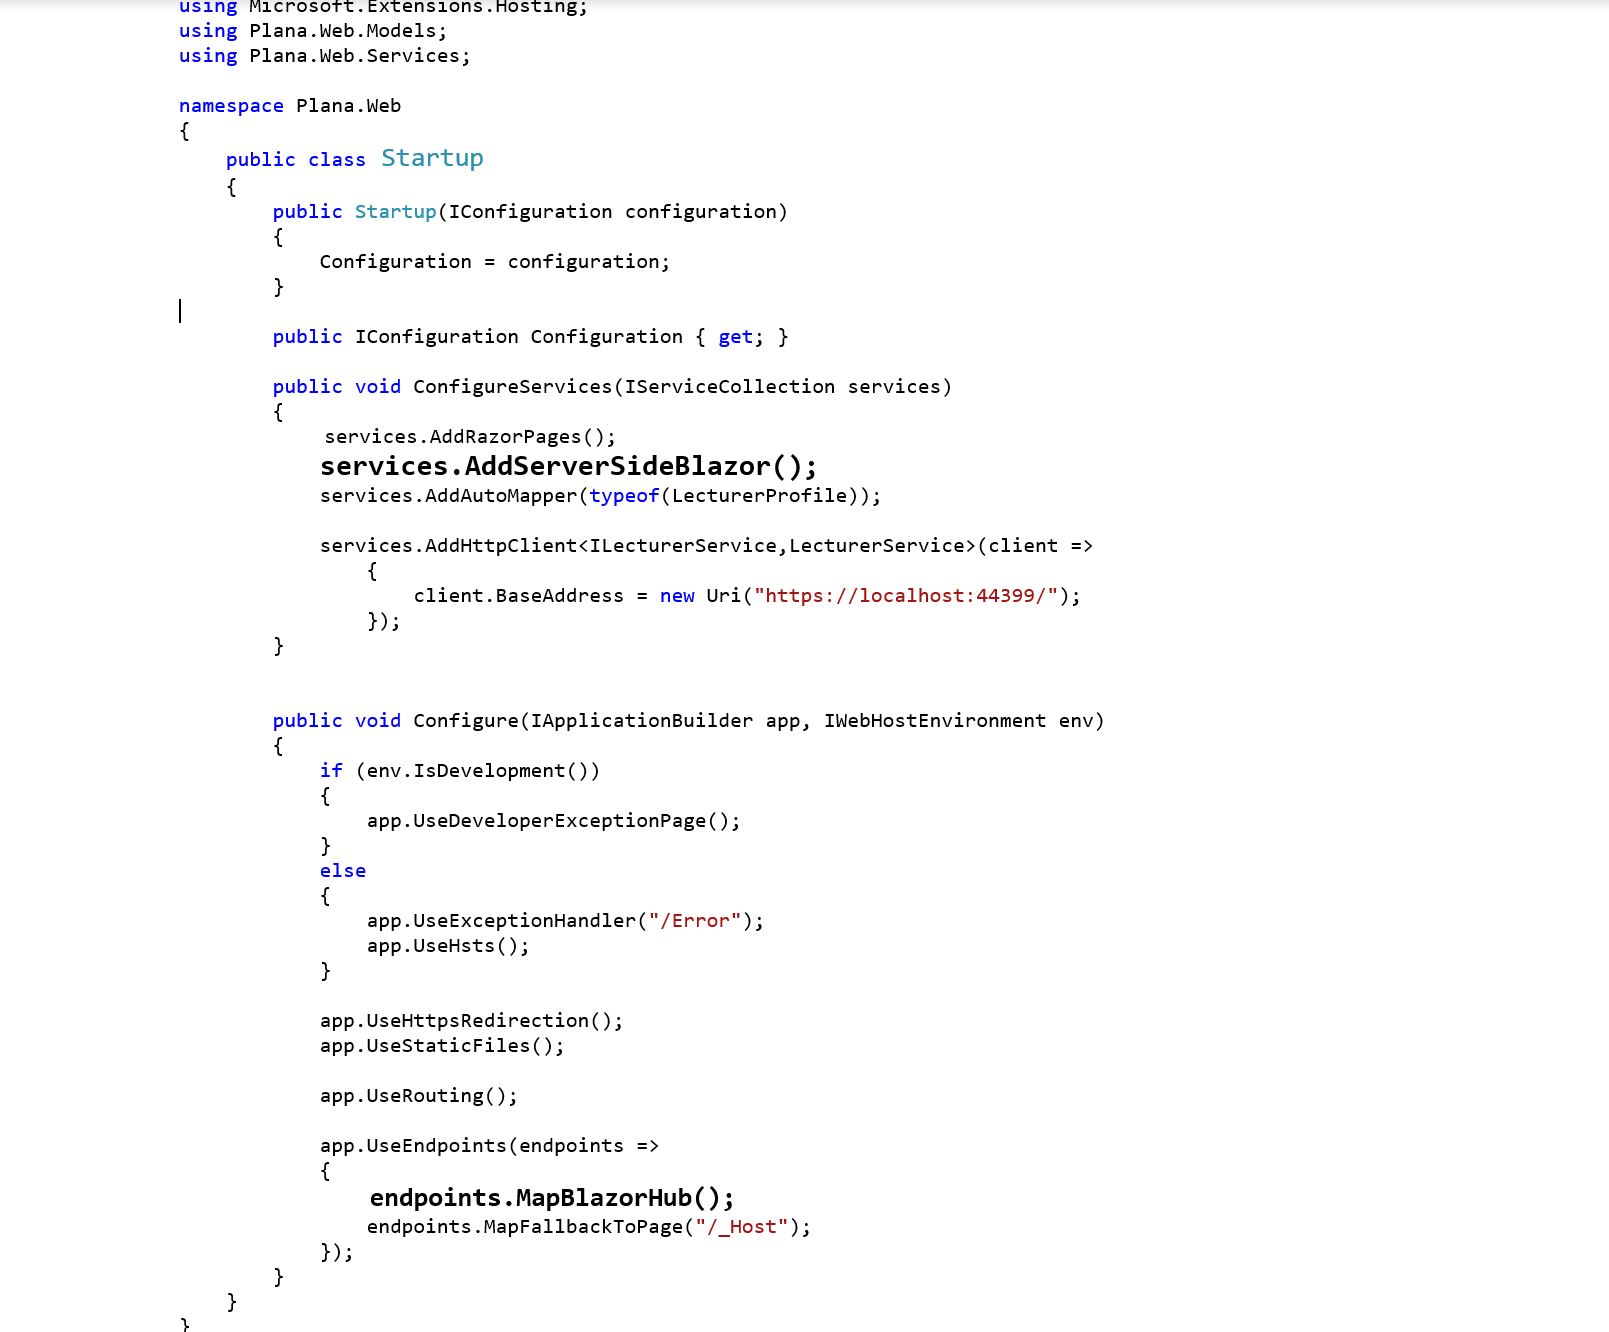
\includegraphics[keepaspectratio=true,scale=0.9]{report_img/add-blazor-service-to-startup}}
\captionof{figure}{Adding Services and Middleware in the Startup.cs File in the Plana.Web project folder}
\label{visina8                                                      }
\end{minipage}

\newpage

When we need to use some data from other folders in a blazor files like Razor files(.razor) all necessary imports we include in the partial class \textbf{ \_Imports.razor} using the \textbf{@using} directives.\\ 


\noindent                                                                
\begin{minipage}{\linewidth}                           
\makebox[\linewidth]{                                      
  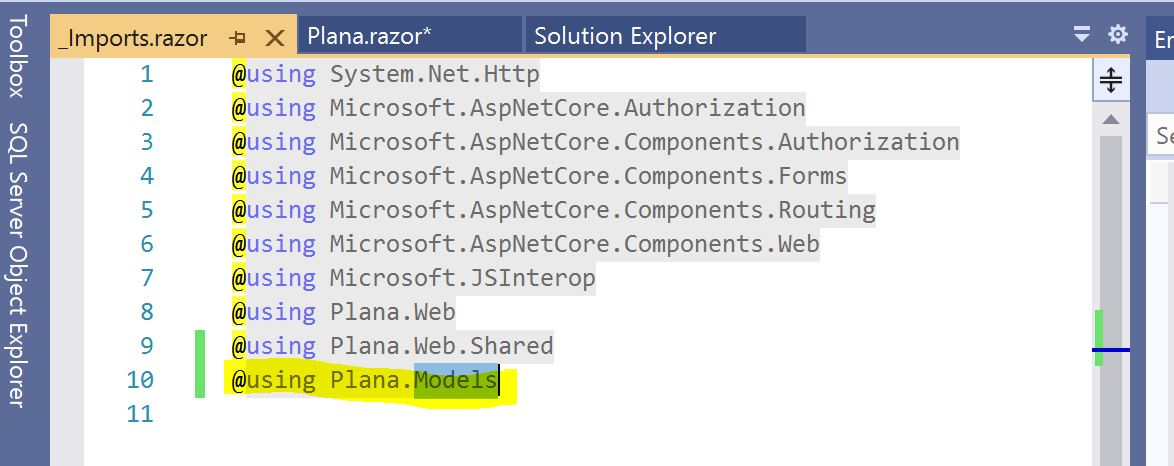
\includegraphics[keepaspectratio=true,scale=0.9]{report_img/blazor/imports_razor}}
\captionof{figure}{Adding required namespaces to the \_Imports.razor file in Plana.Web project folder}
\label{visina8                                                      }
\end{minipage}

\subsection{Setup for Blazor}
To use the Blazor framework it is necessary to install :\\
\begin{itemize}
\item \textbf{.NET Core SDK 3.1 or later} from \url {http://dotnet.microsoft.com/download}
\item \textbf{Visual Studio 2019} from \url {https://visualstudio.microsoft.com/downloads/}
\end{itemize}

%\section{Proof of Concepts }
%/**
%determine whether an idea can be turned into a reality\\
%test if the idea is viable and explore 
%\\
%how the proposed product or service will support organizational goals\\
%*/







%\section{Work Plan}
  		
  		
	The sprints covered a one three-four weeks period. At the end of each sprint, there was a discussion with the supervisor.
%
%In Table 11 is an overview of what was achieved in which sprint.
%\textbf{Sprint's Backlog}
%
%\begin{table}[H]
%\begin{center}
%\begin{tabular}{| p{1cm}|p{3cm}|p{7.5cm}|p{2.5cm} |p{2.5cm} |}
%\hline
%\rowcolor{LightCyan}
%\textbf{ID} & \textbf{Task Name} & \textbf{Task Description}  & \textbf{Priority} & \textbf{Status}\\
%\hline
%
%1                   &        & & & trtwt      
%\begin{itemize}
%\item 
%\item
%\item
%
%
%
% \end{itemize}\\ \hline
% 
%2                &     & & &                
%\begin{itemize}
%\item 
%\item
%\item
%
%
% \end{itemize}\\ \hline
% 3                 &     & & &                  
%\begin{itemize}
%\item 
%\item
%\item
%
%
% \end{itemize}\\ \hline
% 4                  &     & & &               
%\begin{itemize}
%
%\item 
%\item
%\item
%\end{itemize}\\ \hline
% 
%  5            &     & & &                 
%\begin{itemize}
%
%\item 
%\item
%\item
%
% \end{itemize}\\ \hline
% 
%
% 
% 
%
% \end{tabular}
%\end{center}
%\caption{Sprint Backlog of Sprints}
%\label{table2}
%\end{table}
%
%\pagebreak
%
%\begin{table}[H]
%\begin{center}
%\begin{tabular}{| p{1cm}|p{3cm}|p{7.5cm}|p{2.5cm} |p{2.5cm} |}
%\hline
%\rowcolor{LightCyan}
%\textbf{ID} & \textbf{Task Name} & \textbf{Task Description}  & \textbf{Priority} & \textbf{Status}\\
%\hline
%
%6                &     & & &        
%\begin{itemize}
%\item 
%\item
%\item
%
%
% \end{itemize}\\ \hline
% 
%  7                &     & & &                 
%\begin{itemize}
%\item 
%\item
%\item
% \end{itemize}\\ \hline
% 
%  8                 &     & & &                 
%\begin{itemize}
%\item 
%\item
%\item
%
%\end{itemize}\\ \hline
%
%  9                 &     & & &                  
%\begin{itemize}
%\item 
%\item
%\item
% 
%\end{itemize}\\ \hline
% 
%  10               &     & & &                 
%\begin{itemize}
%\item 
%\item
%\item
%
%
% \end{itemize}\\ \hline
% 
%  11                &     & & &                 
%\begin{itemize}
%\item 
%\item
%\item
%
% \end{itemize}\\ \hline
% 
% 
% \end{tabular}
%\end{center}
%\caption{Sprints}
%\label{table2}
%\end{table}
% 
% 
% \pagebreak
%\begin{table}[H]
%\begin{center}
%\begin{tabular}{| p{1cm}|p{3cm}|p{7.5cm}|p{2.5cm} |p{2.5cm} |}
%\hline
%\rowcolor{LightCyan}
%\textbf{ID} & \textbf{Task Name} & \textbf{Task Description}  & \textbf{Priority} & \textbf{Status}\\
%\hline
% 
%  12               &     & & &                  
%\begin{itemize}
%\item 
%\item
%\item
% 
%
% \end{itemize}\\ \hline
% 
%  13                &     & & &                  
%\begin{itemize}
%\item 
%\item
%\item
%
%
% \end{itemize}\\ \hline
%  14               &     & & &                   
%\begin{itemize}
%\item 
%\item
%\item
%\end{itemize}\\ \hline
% 
% 15                 &     & & &                  
%\begin{itemize}
%
%\item 
%\item
%\item
%
%
% \end{itemize}\\ \hline
% 16               &     & & &                  
%\begin{itemize}
%\item 
%\item
%\item
%
%
% \end{itemize}\\ \hline
% 17               &     & & &                   
%\begin{itemize}
%\item 
%\item
%\item
%
% \end{itemize}\\ \hline
% 
%\end{tabular}
%\end{center}
%\caption{Sprints}
%\label{table2}
%\end{table}

\section{Testing}

\section{Summary}
%   \subsubsection{Summary}
\subsection{Conclusions}
\subsection{Future Work}
\subsection{Lessons Learned}

\section{List of illustrations}
\section{Contents of the table}
\section{Appendix}
\section{Declaration of Authorship}
I hereby certify that I composed this work completely unaided, and without the use of any other sources or resources other than those specified in the bibliography. All text sections not of my authorship are cited as quotations, and accompanied by an exact reference to their origin.\\
\\
Place, date:\\
\\

Signature:


\newpage

%% print the bibliography and add the section to the table of content

\printbibliography[heading=bibintoc]


\pagebreak









  	
  
  	

  	
  	
  	
  
  	
  	
  	
  
  	
  	
  
  	


  	





	
	
	




 









 

 























                      
        
    


   

   
    
   
  

\section{Protocol}
\textbf{\textit{Frequency: (biweekly) \\
Meeting length: (60 minutes)}}\\

Agenda

\begin{itemize}
  	\item Demo and Discuss Deliverable(Demo)
  	\item Planning next Goals(Plan)
  	\item Retrospective
  	\item Date, time of the next meeting(next meeting)
 \end{itemize} 	


\textbf{\textit{Report from 24.09.20  }}\\
Plan\\
Future goals are: 
\begin{itemize}


	\item 
	\item 
\end{itemize}	
Retrospective\\

Next Meeting: 08.09.20\\
\**** \\
%%%%%%%%%%%%%%%%%%%%%%%%%%%
\textbf{\textit{Report from 08.10.20  }}\\
Plan\\
Future goals are: 
\begin{itemize}


	\item 
	\item 
\end{itemize}	
Retrospective\\
 
Next Meeting: 21.10.20\\


\****
%%%%%%%%%%%%%%%%%%%%%%%%%%%%

\textbf{\textit{Report from 21.10.20(13:30)  }}\\
Plan\\
Future goals are: 
\begin{itemize}
    \item Implementation. Add new concept classes into the application. 
  	\item  Implementation. Start implementation of graphic concepts we've made.
	\item Make Study director plan view concept with less elements.
	\item Put UI concepts to the report.
\end{itemize}	
Retrospective\\
\begin{itemize}
\item In graphical concept i have choice between semester view and year view, but for planning is more important year view.
\item Actual state of planing view for study director looks little bit heavy because of many elements in it, would be better to minimize some staffs. In implementation we can manipulate view hiding some part of them. 

\item Additional Assignments have a category, description and number of hours.

\end{itemize}
Next Meeting: 04.11.20 (13:30)\\


\****
%%%%%%%%%%%%%%%%%%%%%%%%%%%%

\textbf{\textit{Report from 04.11.20  }}\\
Plan\\
Future goals are: 
\begin{itemize}
  \item \textbf{report} Describe the Additional Assignments. There are several Arts of Additional Assignments. The Lecturer and also Study Director can plan and manage it.
  \item \textbf{report} Describe what is innovative in this work. For example that Lecturer, Study Director and Institute Manager can active collaborate with each other. That is idea of making groups is also innovative. In general, we make a specific solution for problem that we face.
  \item Put tasks which have to be done until \textbf{21-January 2021} into the sprint backlog. These are 
  \begin{enumerate}
  \item Report
  \item Final Presentation
  \item Book
  \item Video
  \end{enumerate}
\item \textbf{Application} Implement the views that we made with Axure tools.
\end{itemize}	

Retrospective\\
\begin{itemize}
\item The graphical concepts looking better now.
\item Conflict between number of hours and lecturers that can teach specific module have to be in application.

\end{itemize}
Next Meeting: 18.11.20 (13:30)\\

\****
%%%%%%%%%%%%%%%%%%%%%%%%%%%%

\textbf{\textit{Report from 18.11.20  }}\\
Plan\\
Future goals are: 
\begin{itemize}
  \item 
\end{itemize}	
Retrospective\\
\begin{itemize}

\item
\end{itemize}
Next Meeting: )\\

\****
%%%%%%%%%%%%%%%%%%%%%%%%%%%%

\textbf{\textit{Report from  }}\\
Plan\\
Future goals are: 
\begin{itemize}
   \item
\end{itemize}	
Retrospective\\
\begin{itemize}
\item

\end{itemize}
Next Meeting: )\\


\end{document}





